\documentclass[a4paper, 10pt, notitlepage]{report}
%===================Package Area==================%
\usepackage[top=2.54cm, bottom=3.89cm, foot=1cm, left=3.17cm, right=3.22cm]{geometry}
\usepackage[CJKnumber]{xeCJK}
\usepackage{fontspec}
\usepackage{indentfirst}
\usepackage{abstract}
\usepackage[bf,small,indentafter,pagestyles]{titlesec}
\usepackage{fancyhdr}
\usepackage{graphicx}
\usepackage{setspace}
\usepackage{titletoc}
\usepackage{enumerate}
\usepackage{enumitem}
\usepackage{amsmath}
\usepackage{subfigure}
\usepackage{natbib}
\usepackage{listings}
\usepackage{xcolor}
%===============Font Settings==================%
\newcommand\fontnamehei{STHeiti}
\newcommand\fontnamexihei{STXihei}
\newcommand\fontnamesong{STSong}
\newcommand\fontnametimes{Times New Roman}
\newcommand\fontnamemono{Courier New}
\renewcommand{\sfdefault}{\fontnamehei}
\setCJKmainfont[BoldFont=\fontnamehei]{\fontnamesong}
\setromanfont{\fontnametimes}
\setCJKsansfont[BoldFont=\fontnamehei]{\fontnamexihei}
\newfontfamily{\HEI}{\fontnamehei}
\setmonofont[Scale=0.8]{\fontnamemono}
\XeTeXlinebreaklocale "zh"
\XeTeXlinebreakskip = 0pt plus 1pt

\newcommand{\sanhao}{\fontsize{15.75pt}{\baselineskip}\selectfont}
\newcommand{\sihao}{\fontsize{14pt}{\baselineskip}\selectfont}
\newcommand{\xiaosihao}{\fontsize{12pt}{\baselineskip}\selectfont}
\newcommand{\wuhao}{\fontsize{10.5pt}{\baselineskip}\selectfont}
\newcommand{\xiaowuhao}{\fontsize{9pt}{\baselineskip}\selectfont}
\newcommand{\liuhao}{\fontsize{8pt}{\baselineskip}\selectfont}

%================段落设置===================%
\renewcommand{\baselinestretch}{1.20}
\setcounter{secnumdepth}{3}
\setlength{\bibsep}{0.5ex}
\setlength{\parindent}{2em}
\setlength\absleftindent{0pt}
\setlength\absrightindent{0pt}

\renewcommand{\labelenumi}{(\theenumi)}
\renewcommand{\figurename}{图}
\renewcommand{\bibname}{\sffamily\mdseries 参考文献}
\newcommand{\supercite}[1]{\textsuperscript{\cite{#1}}}
\renewcommand{\contentsname}{\sffamily\mdseries\sanhao 目\quad 录}
\titlecontents{chapter}[0pt]{\addvspace{0pt}\filright\wuhao}
              {\contentspush{第\CJKnumber{\thecontentslabel}章\ }}
              {}{\titlerule*[4pt]{-}\contentspage}
\titlecontents{section}[0pt]{\addvspace{0pt}\filright\wuhao}
              {\contentspush{\quad\ \ \ \thecontentslabel\ }}
              {}{\titlerule*[4pt]{-}\contentspage}
\titlecontents{subsection}[0pt]{\addvspace{0pt}\filright\wuhao}
              {\contentspush{\qquad\quad\ \thecontentslabel\ }}
              {}{\titlerule*[4pt]{-}\contentspage}

\titleformat{\chapter}{\centering\sanhao\bfseries}{第\CJKnumber{\thechapter}章}{1em}{}
\titlespacing*{\chapter}{0pt}{0pt}{40pt}
\titleformat{\section}{\sffamily\mdseries\sihao}{\thesection}{4mm}{}
\titlespacing{\section}{2em}{16pt}{14pt}
\titleformat{\subsection}{\normalfont\xiaosihao}{\thesubsection}{4mm}{}
\titlespacing{\subsection}{2em}{12pt}{8pt}
\titleformat{\subsubsection}{\normalfont\xiaosihao}{\thesubsubsection}{4mm}{}
\titlespacing{\subsubsection}{2em}{0pt}{0pt}

\titleformat{\paragraph}[runin]{\normalfont\xiaosihao\bfseries}{\theparagraph}{0pt}{}
\titlespacing{\paragraph}{0pt}{1.25ex plus 0.5ex minus 0.25 ex}{0.5ex}

\lstset{
keywordstyle=\color{blue!70}, commentstyle=\color{red!50!green!50!blue!50},
frame=shadowbox,
rulesepcolor=\color{red!20!green!20!blue!20}
}

%==============页眉页脚设置================%
\setlength{\headheight}{1.5cm}
\fancypagestyle{plain}{
	\fancyhf{}
	\pagestyle{fancy}
	\lhead{\includegraphics[width=4.27cm]{logo.png}}
	\rhead{\xiaowuhao 数字图像的真实性检测}
	\cfoot{\liuhao 第\,\thepage\,页~~共\,\pageref{lstpage}\,页}
%	\cfoot{}
}
\fancypagestyle{myheadings}{
	\fancyhf{}
	\pagestyle{fancy}
	\lhead{\includegraphics[width=4.27cm]{logo.png}}
	\rhead{\xiaowuhao\bfseries 数字图像的真实性检测}
%	\cfoot{第\,\thepage\,页~~共\,\pageref{lstpage}\,页}
	\cfoot{}
}
\pagestyle{fancy}
\lhead{\includegraphics[width=4.27cm]{logo.png}}
\rhead{\xiaowuhao\bfseries 数字图像的真实性检测}
\cfoot{\liuhao 第\,\thepage\,页~~共\,\pageref{lstpage}\,页}
\AtBeginDocument{\addtocontents{toc}{\protect\thispagestyle{myheadings}}}
%=================titlepage=====================%
\begin{document}
\fontsize{10.5pt}{13pt}\selectfont%

\chapter*{数字图像的真实性检测}
	\thispagestyle{myheadings}
	\renewcommand{\abstractname}{\sihao\sffamily\mdseries 摘要}
	\begin{abstract}
	\wuhao
	\vspace{25pt}
	随着现代数字图像处理工具的日渐完善,如Photoshop等常用的数字图像处理工具已经拥有的内容感知功能,每个人可以轻易抹去图像上的某些部分来达到修改图像的目的。这促使了数字图像取证技术的发展。但是目前有没有既定的方法,以验证数字图像的真实性和完整性。数字图像取证是新兴的具有重要影响研究领域。

	本文从数字图像的压缩方式、图像采样设备的痕迹、数字图像本身的特定属性等方面,研究了数字图像主要的伪造方式及其对应的鉴别方式。数字图像的伪造通常分为合成图像,变体图像,润饰图像,增强图像,计算机生成图像以及绘图图像等类别。针对数字图像中移动粘贴(使用照片中特定的部分经过重采样,图像调整,加入一定的噪音或随机化处理后复制移动等)的伪造方式,选择针对该方式双重JPEG压缩检测算法,基于SIFT算法的复制移动图像检测算法,基于EM算法的重采样检测等算法进行深入分析,通过比较算法的时间复杂度,适用对象,检测成功率和实际效率来综合各个算法的适用范围。

	经过深入分析比较,我们总结出数字图像取证技术中针对复制粘贴(拼接)图像真实性鉴别的一般方式,即双重JPEG压缩的初步检测和基于SIFT算法的深入检测相互结合。实现通过基于图像直方图的傅立叶变换及DCT系数的傅立叶变换的双重JPEG压缩检测算法和Robust复制移动检测算法的综合方法。

	\end{abstract}

	\vspace{16pt}
	\paragraph{关键词:}
	数字图像取证,图像伪造,JPEG二次压缩检测算法,复制移动检测算法,设备一致性,自然图像一致性


\chapter*{DIGITAL IMAGES AUTHENTICITY DETECTION}
	\thispagestyle{myheadings}
	\renewcommand{\abstractname}{\sihao ABSTRACT}
	\begin{abstract}
	\wuhao
	\vspace{20pt}
	With modern digital image processing tools are improved, it has never been so easy to manipulate images. The Adobe Photoshop's content-aware feature which was allowed everyone to erase some parts of the image to achieve the purpose of hiding some information from the original. This has prompted the development of a digital image forensics. However, there are no established method to verify the authenticity and integrity of most digital images. The digital image forensics is an emerging research field.

	The forgery digital images are usually divided into the composited images, morphed images, retouched images, enhanced images, computer-generated images and drawings. In this paper we introduce methods to detect Copy-Paste forgery in digital images. The histograms of DCT coefficients of a double compressed image contain specific periodic artifacts detectable in the frequency space. The SIFT algorithm to detect the Copy-Move. The consistency of statistical characteristics of natural images.

	 After in-depth analysis of the comparison, we summed up the general way in the digital image forensics technology for copy and paste (mosaic) image Authenticity relies on the double JPEG compression detection algorithm based on the fourier transform of the image histogram and DCT coefficients  and Robust Copy-Move detection algorithm.

	\end{abstract}

	\vspace{20pt}
	\paragraph{Key words:}
	Digital image forensics, Image Forgery, Natural image consistency, Authenticity detection


\tableofcontents \thispagestyle{myheadings}


%================content===================%
\chapter{绪论}
	\setcounter{page}{1}
	历史总是在真相和谎言之间徘徊,历史上政治意味的照片总是充满了被篡改的痕迹,一次又一次颠覆了对图像完整性的信任。从19世纪相机被发明出来之后,这种篡改真相的行为就没有停止过。从初期对胶片的修改,到如今数字化时代彻底削弱这种对照片媒介信任,针对数字图像的攻击行为传达了一个不存在的场景或对象的描述,到目前为止都没有很好保障措施的来验证这种视觉证据的完整性和真实性\supercite{overview01}。

	数字取证领域的出现,就是为了帮助恢复对数字图像完整性和真实性的信任。
	
	\section{数字图像取证的背景}
		在数字图像广泛应用的今天,随着Photoshop、Paint.NET等高质量图像工具的出现,修改一张数字图像变得愈来愈容易,也更难辨真伪。过去那些因为政治因素而需要一个团队花上十几个小时手工修改照片的情形在如今变的无比简单。如何辨别一张重要照片的真伪成为了一个新的发展趋势。中国国家地理杂志的摄影师曾因为虚假照片的获奖而不得不辞职\supercite{sa02},政府也不得不出面为他的行为道歉。另外,曾被广泛报道的伊拉克女记者丑闻的照片却被发现是一场政治陷害。

		\begin{figure}[ht]
			\centering
			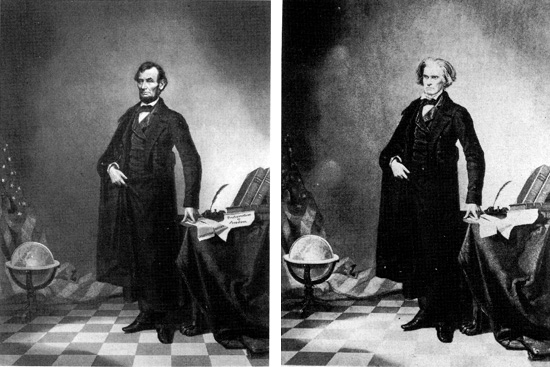
\includegraphics[width=5in]{img/c1860-Lincoln.jpeg}
			\caption{Abraham Lincoln}
			\label{fig-lincoln}
		\end{figure}

		图\ref{fig-lincoln}显示这张标志性的美国总统亚伯拉罕·林肯的肖像(版画的形式)是一个林肯的头和南部的政治家约翰·卡尔霍恩的身体的复合照片。

		\begin{figure}[ht]
			\centering
			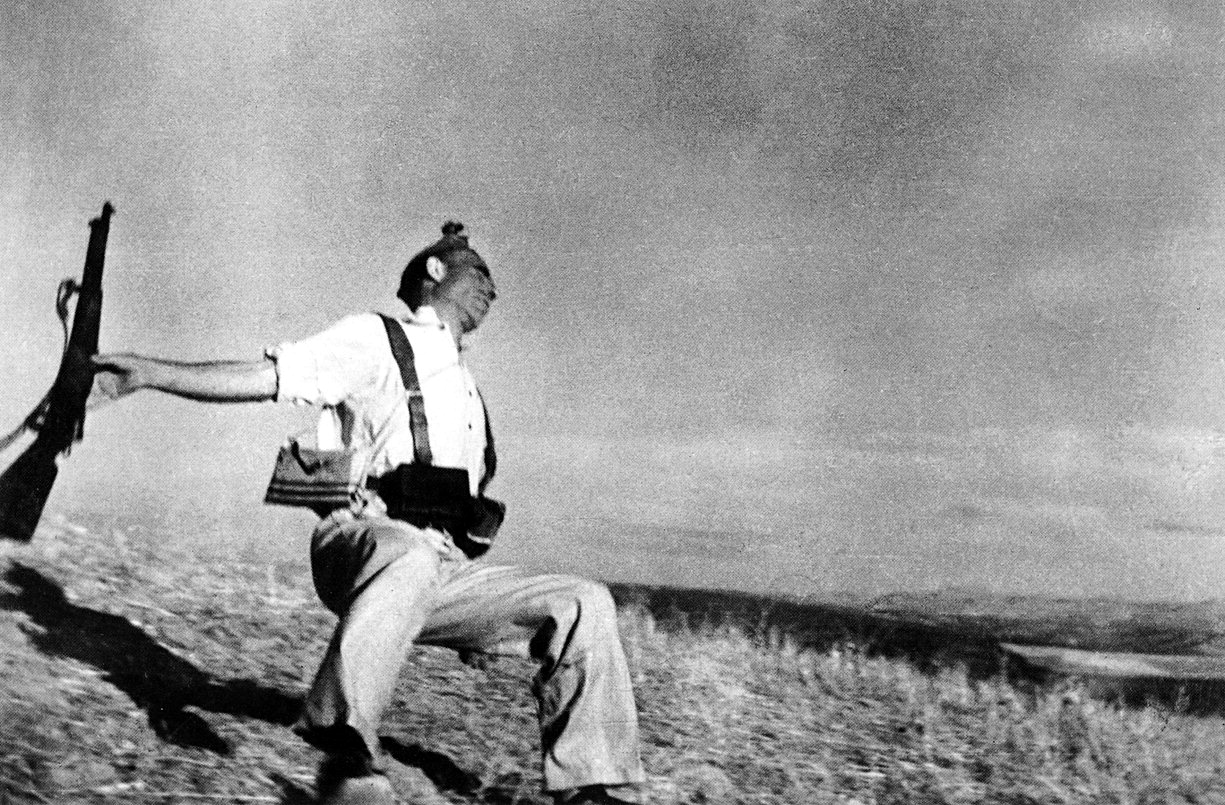
\includegraphics[width=5in]{img/capa_thefallingsoldier.jpeg}
			\caption{罗伯特·卡帕 倒下的士兵(1936)}
			\label{fig-capa}
		\end{figure}

		罗伯特·卡帕(Robert Capa)著名的摄影作品,坠落的士兵(The Falling Soldier 1936, 如图\ref{fig-capa}所示),可能是最新加入的艺术假照片。照片描绘的是1936年在西班牙内战中的士兵,在他去世的时刻,扭曲地倒向地面,步枪从他手中滑落。但西班牙研究员何塞·曼努埃尔(Susperregui)在他的一本新书《摄影的阴影》中表明,这张照片并不取景于摄影师所说的地点。在西班牙媒体的帮助下,他设法匹配照片的位置并不在当时的战场埃斯佩霍。历史学家而后添加了更多的证据:在埃斯佩霍的战斗还没有开始时,卡帕就已经拍摄了这张照片。

		\begin{figure}[htp]
			\centering
			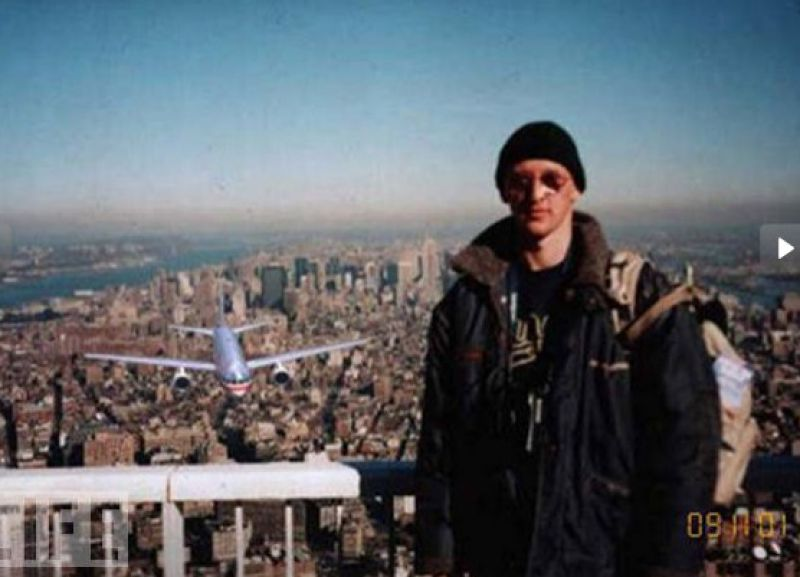
\includegraphics[width=5in]{img/19025168_3.jpeg}
			\caption{911恐怖袭击假照片}
			\label{fig-911}
		\end{figure}

		图\ref{fig-911}在911恐怖袭击之后,一幅男人站在世贸大厦天台,背景是即将撞楼的飞机,右下角还有911的日期的照片,迅速走红网络。但很快又有人指出包括飞机飞来的方向、飞机类型、阳光在飞机上的反光、以及拙劣的日期更改痕迹都显示出伪造的迹象。不过最大的证据就是,如果是真有人拍照,那么在几秒钟后的恐怖袭击后,这张照片还能够存在的可能性非常低。最后,照片中的人出面承认是他和几个朋友拿自己的某张照片篡改的,不过没想到会传播的这么广。

		一张张真假难分的争议照片在微博等社交媒体上快速传播,很多负面影响难以被消除。在越来越多的场合,这促使了数字图像取证技术的发展。目前有没有既定的方法,以验证数字图像的真实性和完整性。数字图像取证是新兴的具有重要影响研究领域。

		图像媒体在法庭上总是会被作为重要的证据所采用。无论是民诉中证据的类型,还是刑诉中证据的类型或者行政诉讼法中的证据都包含书证和视听材料等部分\supercite{魏振瀛2007民法}。图片只是一种载体,通过它记录的内容来确定其是书证还是视听资料,如果图片记录的内容本身就能直接证明案件事实,那他就是书证。如果图片中的内容是一个具体的物或者文书,或者其它,而是这些内容包含的信息来证明案件事实,则其应该为视听资料。如果照片证明的事实有其它证据能够相互印证,那么证据被采纳的可能性就大。这种影响的背后,就导致伪造图像作为假证据破坏法庭信誉的行为。这些针对图像的攻击行为可能直接改变了现实生活中的事件和对象的描述。

		尤其是当它涉及到法律的摄影证据。法律没有规定作为证据的素材的认证过程,通常是有经验丰富的调查员通过人眼可观察的部分对照片进行分析。但是这种分析往往片面而且难有成效。通常是工作多年经验丰富的检测人员,也有可能败在精心设计的伪装之中。这就好比临摹德加的名画,或者仿制一品百年红酒。如果不是放射性元素检测技术的发展,市场上可能出现更多伪造的艺术品。

		数字图像取证的需求主要是面向三个方面:
		\begin{enumerate}\setlength{\itemsep}{-0.1cm}
			\item 图像源的鉴定。检测图像是由那种成像设备所获得的,如数码相机、扫描仪等。
			\item 检测图像是否和真实的生活场景相符合。
			\item 检测图像中是否经过修改或处理之后和它最初被捕获时不同。
		\end{enumerate}

		数字图像取证包括主动取证(数字签名、数字水印)和被动取证(盲取证)技术。前两者通过对原始照片或摄影器材的预处理达到图像完整性目标。而新兴的盲取证技术则是通过图像本身的特性进行辨别,在多个领域中更具有价值。要了解取证技术,首先就必须了解图像的篡改技术。主要分为合成图像、变体图像、润饰图像、增强图像、计算机生成图像以及绘图图像\supercite{summary01}。

	\section{数字图像取证技术研究意义}
		上述分析可以看到,一张伪造的被广泛传播的图像的社会危害性不言而喻。无论是一张政治照片还是娱乐新闻照片,都可能因为伪造而被推向舆论的风口浪尖。研究数字图像的取证技术,特别是通过非主动手段(数字水印,数字签名)的手段研究数字图像的真实性是一个极其重要的课题。这是对历史的忠诚。还原一个政治事件的真实动机,还原一次战争的最原本的经历,还原一次诉讼案件的真相,还原一次互联网炒作的背后利益。从技术角度上而言,可以提高对图像在密码学上的应用(信息隐写技术发展)。实现对图像完整性和认证性的保障。

	\section{数字图像取证研究现状}
		目前国内该领域还处在探索阶段,较落后于国外。国内的研究目前主要通过图像统计学特征、图像伪造后造成的某些规律的产生或消失,利用一些成熟的数学方法如边缘分析、自然图像和伪造方法产生的差异等进行分析。
	国外目前已有不少基于内容识别的方法,利用人脸、眼球的特殊成像模式、局部光源方向进行处理。在算法研究方面,Dartmouth 学院、Binghamton大学、Columbia大学和美国Polytechnic大学等成立了专门的数字媒体取证研究小组。
	
	\section{本文贡献}
		本文阐述了数字图像取证技术的现状和分类,介绍现有的稳定算法并比较了它们的优缺点。对复制粘贴这种图像伪造手段进行了特别细致的分析。对JPEG二次压缩基于DCT交流系数零均值直方图的周期规律检测算法和Robust复制移动检测算法进行了大量实验和综合分析。

		第一章中主要介绍数字图像取证技术的背景和研究概况。

		第二章介绍了数字图像的基本知识,从图像和成像设备的基本信息,数字图像的主要篡改(攻击)手段和相应的鉴别手段来分析。
	
		第三章着重分析基于复制粘贴的图像伪造鉴别算法,阐述其算法原理。复制移动作为最为常用的数字图像伪造手段,在对象删除、对象增加等方面有很重要的影响。
	
		第四章对比分析二次JPEG压缩算法以及图像内重复内容检测算法的实际效率,并验证对基于复制移动原理进行伪造的图像类型的正确率。通过对比两个算法的实际效率,正确率来明确算法的可用范围。
	
		第五章总结。

	\section{本章小结}
		本章主要介绍了数字图像取证技术的背景及意义,通过分析图像伪造事件及其社会危害性,造成的舆论影响以突出数字图像取证技术的重要性。验证数字图像的完整性和检测篡改的痕迹,而无需使用任何预先提取或预嵌入信息保护已经成为一个重要领域的研究热点。


\chapter{理论基础}
	对于图像取证技术而言,首先要能判断图像是否经过篡改。进一步定位图像的篡改区域,通过何种方式的伪造而得。最后能分析篡改来源,定位其原始图像素材。就目前的图像处理技术来看,主要停留在第一个阶段,即判断图像是否经过篡改。对于部分特定图像及目标算法,可以定位其篡改区域。但是恢复原始图像依然是很困难的行为。

	数字图像对于传统的胶片而言,有更多反应于数据上的数学逻辑和统计学特征。必须知道图像信息包含的内容才能知道其篡改方法和取证手段。作为本篇的理论基础。

	\section{数字图像的基本特征}
		数字图像不同于传统的胶片,由于其本身的数据开放性,借由计算机的强大分析能力,很容易获得远大于人眼所能够获取的信息。

		\subsection{图像的基本信息}
			图像的基本信息包括色彩平衡、色阶、直方图、分辨率、色彩空间、EXIF、数字水印、数字签名等等。
			
			\subsubsection{图像分辨率}
				图像分辨率是用来描述图像细节的属性。无论是数字图像还是影片图像或者其他类型的图片,越高的分辨率意味着更多的图像细节。分辨率有很多种表示方法\supercite{pouliot2002automated},最常见的几种表达如像素分辨率,空间分辨率,光谱分辨率和时间分辨率等。苹果公司在介绍其新iPad时提到其拥有$2048\times1536$的分辨率即是像素分辨率的表达方法,整个9.7英寸的设备上拥有了多达$2048 \times 1536 = 3,145,728$个象素点。但是像素数并不能真正用来表达数码相机的图像分辨率。大部分相机的图像传感器在每个象素点上只能获得一个通道的颜色。然而一张彩色图像的每个象素点至少有红,绿,蓝三种颜色。照相机在将最终图像呈现给用户之前,会对每个象素点的其他两个通道的颜色进行补充,从而呈现较为逼真的图像。这些补全其他两个通道的算法所造成的结果是图像的像素的色彩空间往往具有很多符合统计规律特性。

			\subsubsection{图像的色彩模式}
				色彩模型通常是用三个或三个以上数值表示颜色的抽象数学模型\supercite{stokes1996standard}。如三原色模型(RGB),印刷四分模型(CMYK)等。

				HSB(色相hue,饱和度saturation,明度brightness)则是艺术家常用的色彩表达方法,只是一种更加直观的表达方式而已,从数学模型上看,它只是RGB空间的一种变形。

				YUV色彩模式所描述的是颜色的亮度分量(Y)和色度分量(U和V)。亮度分量代表颜色亮度信息,色度分量包含颜色差异。YUV色彩格式的一个优点是基于人类视觉感知的特点:由于人眼对亮度信息更敏感,色度信息可以被适当降低而不影响视频质量。这种方法被称为色度抽样。所以YUV通常被用来描述视频画面。另外还有YCbCr,YPbPr等色彩模式。其中YCbCr在数字图像和视频处理中,特别是为JPEG图像和MPEG视频编码的所使用。这些色彩模式都可以相互转化\supercite{yang2007fast}。在某些图像伪造鉴别分析中,往往是针对特定色彩空间的某个分量进行分析。

			\subsubsection{色彩平衡}
				色彩平衡是表示图像中颜色的动态范围的术语。在图像处理领域,色彩平衡经常表示通过改变图像的颜色值从而能够在特定的显示或者打印设备上得到正确的颜色\supercite{郑建铧2003利用色彩直方图特征进行偏色图象的自动检测和校正}。数码相机中的白平衡属性即是一种色彩平衡调整方式,白平衡即是相机对白色物体的颜色还原。无论是在日光下,还是在夜晚,人眼所能感知到白色物体始终是白色是因为经过长时间进化后人眼已经对色彩还原有了较好的适应性。

			\subsubsection{EXIF信息}
				EXIF(Exchangeable image file format)是可交换图像文件的缩写,是专门为数码相机的照片设定的,可以记录数码照片的属性信息和拍摄数据\supercite{alvarez2004using}。EXIF信息可以被附加在常见的图片格式(如JPEG, PNG, TIFF)上。但是没有EXIF信息并不表示图像经过篡改,EXIF并不像图片水印一样经过签名或者加密处理,它仅仅作为方便记录图像拍摄数据的存在。

			\subsubsection{RAW格式}
				RAW格式是数字图像的原始图片格式,又称为数字底片。RAW图像格式的目的是尽可能的捕捉(即特定传感器的最好性能)现场的拍摄特性,也就是说,包含有关场景的光照强度和颜色的物理信息。
				\begin{enumerate}\setlength{\itemsep}{-0.1cm}
					\item 更高的图像质量。因为所有的计算(如伽玛校正 ,去马赛克 ,白平衡, 亮度 ,对比度,等等......)用于生成像素值(对于大多数图像的RGB格式)进行一步的基础数据,由此产生的像素值将更加准确,并表现出以下的色调分离 。
					\item 绕过不受欢迎的步骤在相机的处理,包括锐化和降噪等。
					\item RAW格式采用无压缩或使用无损压缩,保存所有的图像细节。
					\item 更精细的控制。RAW转换软件,允许用户操纵更多的参数(如亮度 ,白平衡, 色调 ,饱和度,等等。)。如“日光”或“白炽灯”不只是离散的预设值。用户通常可以通过软件调整这些参数。
					\item 可以设置为任何需要的色彩空间。
				\end{enumerate}
				

			\subsubsection{灰度直方图}
				灰度直方图(histogram)是灰度级的函数,它是图像种不同灰度级的分布函数,是图象的最基本的统计特征。在计算机图像学领域中,灰度直方图常被作为基本的属性分析\supercite{kapur1985new}。

		\subsection{设备特征}
			大部分相机的图像传感器在每个象素点上只能获得一个通道的颜色。Bayer阵列是最常用的色彩滤波器阵列(Color Filter Array, CFA),如图\ref{fig-bayer}。然而一张彩色图像的每个象素点至少有红,绿,蓝三种颜色。相机会从附近的像素差值来补全缺失的通道色,一般的做法是采取相邻数值的平均值,也有一些更复杂的算法,这一过程称为去马塞克。在图像重采样分析中,会具体分析这种类型的特征。

			\begin{figure}[htp]
				\centering
				\includegraphics[width=5in]{img/Bayer_pattern_on_sensor_profile.png}
				\caption{Bayer色彩滤波阵列}
				\label{fig-bayer}
			\end{figure}

			设备还有其他一些特征,如噪点分布等等,不在本文讨论的范畴。
		
		\subsection{图像压缩格式}
			最常见的JPEG格式,利用人类感官对灰度敏感对色度不敏感,从而通过减少色度来达到压缩的目的。利用离散余弦变换、量化和熵编码所得。其后续版本JPEG2000基于拼接块和小波变换,降低方块效应。

			TIFF图像是靠指针连接来组织数据的,文件头和数据可以任意数据的存储。

			便携式网络图形(Portable Network Graphics,PNG)是一种无损压缩的位图图形格式,支持索引、灰度、RGB[A]三种颜色方案以及Alpha通道等特性。PNG使用了从LZ77派生的一个非专利无失真式压缩算法(名为DEFLATE)。这个算法对图像里的直线进行预测然后存储颜色差值,这使得PNG经常能获得比原始图像甚至比GIF更大的压缩率。

	\section{数字图像主要篡改方法}
		要了解数字图像取证技术,首先必须了解数字图像伪造的主要方法。对于一张包含传达虚假信息的照片,通常会对照片中包含的人物、事物、地点等作出改变。最常见的方式有复制移动,包含多个来源的照片拼接,对拼接照片(从源图像中提取的目标对象)的边缘进行模糊,整体的的曲线调整,图像的隐藏信息写入技术等等。都会对图像本身所要传达的信息造成改变。归纳图像的主要伪造方式有助于更好得分析图像特征,归纳不同得取证算法的目标。节省在图像综合性取证技术上的时间,分析其算法特征如高斯模糊甚至可以达到逆向获取原始图像素材的目的。

		\subsection{主要篡改类型}
			合成图像,通过合成不同来源的图像构成新的图像,以传递虚假信息。
			变体图像,对图像上的特征点为基准对图像进行修改\supercite{surveyof}。
			润饰图像,使用滤镜操作修改图像。
			增强图像,调整图像基本参数的行为。
			计算机生成图像以及绘图图像,通常是非照相设备所获取的图像。
		
		\subsection{复制移动}
			复制移动伪造是常见的图像伪造技术之一。攻击者复制源图像本身的一部分,将其粘贴到目的图像的另一部分,来掩饰一些图像细节的目的。通常有几种常见的应用情形,比如同一张图片内的目标元素的隐藏、目标元素的增加,又如不同图片之间的复制和粘贴。后者通常会带来更多可被检测的属性,因为要契合两张不同尺寸的图像必然需要对图像本身进行平移、旋转等尺度变化,这种特定的变化已经可以被检测出来。尽管从表面上看,人眼只能观察到图像很小的一部分信息,对于图像背后数字的符合统计学特征的规律只能通过计算机分析才能得到。

			复制移动的目的有为了消除背景中的某些对象,通过移动周围背景的纹理达到伪造的目的,也有为了复制更多在背景中的对象,而提取对象的图层进行平移、翻转、缩放、旋转等操作。也会有将不同来源的照片拼接而成。常见的电影海报就是这种方式。

			如著名数字图像处理软件Photoshop所提供的图章工具,可以用来选取图像上特定的部分作为笔刷进行填充,常用来修复皮肤,去除不需要的噪点等等。还有其内容感知工具(Content-Aware),更是可以智能分析图像中的背景,其原理是基于色彩梯度的分析找出选择的范围中物体的边界,利用该物体周围的背景图像的复制和移动达到去除图像中特定元素的目的,该工具还可以用来创建多个相同元素的拷贝以达到某些特定的效果。文\supercite{ding2010content}中指出,对于图像智能感知的研究通常基于两方面:一是图像的剪切,指从源图像提取要复制的对象;二是图像的粘贴,将对象粘贴到目的图像上。对于粘贴区域的处理通常有两种方式,一种是执行一个简单的alpha通道混合方法(即对源图像和目的图像交叉的部分做函数变化),这种方法并不适用与所有情形,如果对象周围的颜色较为复杂,简单的混合模式不能完成任务;另一种方法则是对图像边缘进行羽化,寻求尽可能自然的过渡方式。

		\subsection{人工模糊}
			在图像伪造过程中,模糊操作是最常用的操作之一。伪造者通常会在图像拼接后采用模糊、淡化、渐变等润饰操作以消除简单拼接留下的伪造痕迹。模糊操作的基本原理是对图像的局部邻近像素值进行邻域灰度平均,其目的是为了消除图像伪造在拼接边缘产生的视觉或统计上的畸变。识别人工模糊是图像取证至关重要的一项。Photoshop中包含了场景模糊(Field Blur),焦外模糊(Iris Blur),移轴模糊(Tilt-Shift),高斯模糊(Gaussian Blur),镜头模糊(Lens Blur),动态模糊(Motion Blur),径向模糊(Radial Blur),表面模糊(Surface Blur)等等。

			在边缘处理中,高斯模糊是最常用的处理方式,从数学的角度来看,图像的高斯模糊过程就是图像与正态分布(高斯分布)做卷积。而焦外模糊则是图像与圆形方框模糊做卷积,它会生成更加精确的焦外效果。二维空间的正态分布定义为:
			\begin{equation}
				G(u,v) = \frac{1}{2\pi\sigma^2}e^{-\frac{u^2+v^2}{2\sigma^2}}
			\end{equation}
			对一幅图像进行多次连续高斯模糊的效果与一次更大的高斯模糊可以产生同样的效果,大的高斯模糊的半径是所用多个高斯模糊半径平方和的平方根。

		\subsection{图像隐写}
			隐写术(Steganography)最早被记录在古希腊一本黑魔法书中。人们利用一种特殊德章鱼墨汁作为隐形墨水写在纸上,受热显形。对于数据隐写而言,掩盖数据的容量越大,隐藏越容易。所以,数字图像被广泛用于消息的隐藏。数字图像消息隐写算法主要分时间域(Spatial Domain)和变换域(Transformation Domain)两种\supercite{张亚伟2008图像隐写分析算法研究}。空间域信息隐藏算法通过直接修改载体图像的像素值来嵌入隐藏的信息,例如一个RGB色彩空间中的图像,每个通道的每个色彩都用8位数值表示,但是相邻两个色彩人眼几乎无法分辨。通过对最低比特位进行编码来嵌入信息,被称为最不重要比特位算法(LSB)。Bander等人提出的Patchwork算法克服了LSB算法图像统计特征的不足,对JPEG压缩、FIR滤波及图像裁剪有一定的抵抗力。Chen等人将隐藏信息设计成量化噪声,用量化矩阵进行编码\supercite{chen2006blind}。

			图像隐写技术并不只是一种数字图像伪造技术,它也可以被用来作为数字水印。

		\subsection{色彩平衡、色阶、对比度等基本参数调整}
			相较于图像部分数据的修改会破坏图像CFA差值的统计学特征,部分图像整体曲线的调整仍可能保持这种特性。但并不意味着这类方式(包括色彩平衡的修改、色阶、整体滤镜、对比度调整)就不是一种图像伪造的方式。一张蓝天白云的照片可能通过修改色彩平衡而变成黄昏,一张写实的照片可能因为滤镜而变成一张油画。这种方式可能不会改变某些统计特征,但是很可能会改变另一些特征。图像可能可以接受某些程度上的对比度增强等简单调整操作。这种界线的界定依然是个很模糊的概念。
	
	\section{数字图像鉴定的主要方法}
		数字化信息革命和多媒体安全有关的问题已经产生了篡改检测的几种方法。一般来说,这些方法可以划分为主动和被动,盲目的办法。主动方法可简单的划分为数据隐藏的方法和数字签名的方法。数据隐藏指嵌入辅助数据到图像的方法。这一领域最流行的方法就是数字水印。水印的一个主要缺点是,他们必须在记录图像时写入,或稍后由授权人写入。需要配备专门的相机或对原始图像进行后续处理。在这项工作中着重于检测双重JPEG压缩的图像。这也是针对最常见的复制移动图像伪造方式的最有效的办法之一。检测双重压缩的痕迹,也有助于在其他领域的研究,如图像隐写。双重压缩的图像可以产生一些隐写算法(量化噪音等等)。图像伪造过程中通常使用伪造的图像模糊操作,伪造者可能使用模糊操作隐藏伪造的痕迹,因此人工模糊检测也是伪造图像取证的重要手段。

		\subsection{光影分析}
		由于人眼对明暗相较于色度更加敏感,最初对照片的人工分析都是从光影的分布来看的。文\supercite{sa01}中所提到的几个通过分析光线和阴影分布来鉴定的方法有:
		\begin{enumerate}\setlength{\itemsep}{-0.1cm}
			\item 对局部的光源进行分析。对象明暗的分布可以指示光源是如何分布的。一张精心安排的照片至少有三束以上的光线,包括主照明(Key Light),补充光线(Fill Light)和背景光(Back Light)。主照明则作为最重要的光源判断依据,物体表面的光量取决于表面光源的相对方向。对于自然环境光线的照片而言,反向的阴影往往意味着照片中存在有其他图片源的部分。
			\item 眼球位置。每个人眼睛有非常一致的形状,从虹膜的形状可以推断一个人是如何面对相机的。通过相机的位置和场景是否符合来作为图像是否经过篡改的证据,如图\ref{fig-eye}。
			\item 镜面高光。周围灯光反映在眼球上,形成小的白点被称为镜面高光。这些亮点告诉我们照明的位置。实际上和方法一是类似的,不过方法一主要通过阴影,而人眼是有一些不同的特质。往往多人组合的宣传照片可以通过这种方法来判断。
		\end{enumerate}
		%=================== figure 1 ===================%
			\begin{figure}[ht]
				\centering
				\subfigure[]{
					\includegraphics[width=2.5in]{img/eyes.jpg}
					\label{fig-eye:subfig1}
				}
				\subfigure[]{
					\includegraphics[width=2.5in]{img/eyes2.jpg}
					\label{fig-eye:subfig2}
				}
				\subfigure[]{
					\includegraphics[width=5in]{img/iris.jpg}
					\label{fig-eye:subfig3}
				}
				\caption{\subref{fig-eye:subfig2}虹膜的聚焦方式 \subref{fig-eye:subfig3}虹膜构造}
				\label{fig-eye}
			\end{figure}
		可以看到以上方法主要是明暗分析。人类可以很容易感知人像,而计算机在这方面却缺乏先天的优势。通过程序判断人眼的位置或是眼球的方向并不是一个最好的选择。因为计算机所能看到的远远大于人眼所能得到的明暗和色度的数据。机器分析色彩背后数字的关联性和统计学特征,分析图像函数的特性来抓住重要证据。

		\subsection{数字水印和数字签名}
			数字水印和数字签名的产生主要是对多媒体内容进行两方面的保护:一是版权保护,二是内容完整性保护。传统密码学中的认证方法要求不能对原文有任何修改,需要保存额外的认证信息。而多媒体数据则往往可以容忍一定程度上的失真(人眼无法识别的差异),互联网上常见的多媒体内容引用都是直接引用,数字水印由此诞生\supercite{forgerydetect01, 孙圣和2004数字水印技术及应用, 杨义先2006数字水印理论与技术}。数字水印将一些标示信息直接嵌入多媒体载体中,而不影响载体在人类知觉器官下的感知。数字水印特性主要要求有:
			\begin{enumerate}\setlength{\itemsep}{-0.1cm}
				\item 鲁棒性。利用这种水印技术要求其能在信道噪声、滤波、数/模与模/数转换、重采样、剪切、位移、尺度变化以及有损压缩编码等环境中生存,具有较好的抗攻击能力。当媒体内容发生改变时,数字水印也发生改变。通常会被用于版权保护的作品。它会嵌入作品创建者的个人信息,以及授权许可信息等,当发生版权纠纷时能提供有力的证据。目前尚无十分有效的鲁棒算法。
				\item 隐藏性。数字水印是信息隐藏技术的一个重要研究方向。嵌入数字图像中的水印不易被觉察,且不会引起明显降质。
			\end{enumerate}
			许多实际情况要求在不依赖任何预嵌入信息或签名的前提下,对图像的真伪和来源进行鉴别,本文所探讨的主要是数字图像的盲取证技术。

		\subsection{基于图像伪造过程的遗留痕迹}
			
			\subsubsection{JPEG二次压缩检测}
				JPEG是大多数照片的主要传播格式。合成的图像采用不同片源的JPEG图像再进行第二次压缩,这种双重JPEG压缩会带来新的统计学特征,其DCT系数会满足一定的周期规律。如果不同照片源本身的JPEG压缩质量不同,从一定概率上还能定位篡改区域,目前是研究比较多也是比较成熟的方式。

			\subsubsection{人工模糊检测}
				人工模糊是图像润色主要的方法。人工模糊和相机离焦模糊最大区别在于人工模糊有明确的模糊边界,在模糊边界内外的图像像素相对于模糊的概念区别较大,而相机离焦模糊没有模糊边界,较人工模糊会表现得更加均匀。根据模糊边界灰度是否均匀来判断是否经过人工模糊。

			\subsubsection{复制移动(重复内容)检测}
				通过SIFT算法\supercite{huang2008detection},Robust检测算法\supercite{popescu2004exposing},Bloom过滤器等可以非常准确地检测重复区域的图像,即使复制的地区发生了严重的图像操作。

				\begin{figure}[ht]
					\centering
					\includegraphics[width=5in]{img/content_aware.png}
					\caption{Photoshop 中的内容感知工具只需要简单地框选需要删除的元素,然后选择使用内容感知的方式填充删除区域,软件就会用周围的景象经过一定的变换来填充被删除区域。}
					\label{fig-contentaware}
				\end{figure}

				图\ref{fig-contentaware}是Photoshop中内容感知工具的示例。

			\subsubsection{重采样检测}
				原始自然图像的灰度级是自然变化的。而经过缩放等重采样操作会因为差值等因素产生周期变化。通过EM算法可以找到较好的办法来检测这种类型的改变。


		\subsection{基于成像设备的一致性}
			要了解图像的属性,最好能了解其产生设备。

			数码相机在拍摄过程中,不同镜头的光学畸变不同、不同相机使用的色彩滤镜矩阵 (Color filter array, CFA)和相应的插值算法不同等\supercite{林啟銘2008基於鄰近像素方向資訊之數位相機},这些一致性的规律可用于数字图像伪造检测和篡改定位。区别不同的相机和不同的镜头能更好地对照片进行分析。例如图像中出现多个设备源,就可以认为图像经过了合成处理。这种方法的好处在于还可以定位篡改区域。通过分析图像的背景噪声可以鉴定其生产设备。

			由计算机绘图软件绘制的图像可能会包含笔刷、渐变工具、滤镜等工具所留下的特别痕迹。由于其生产工具的限定,计算机绘图图像会缺乏自然图像所特有的统计特征,也不会拥有那么多细致入微的色彩过渡变化。利用常见的DCT系数分析就可以明显区别其与自然图像的差别。

			基于成像设备一致性的分析是个热门的课题,在本文中不进行深入讨论。
		
		\subsection{利用自然图像的统计特征}
			自然图像数学统计模型一般从图像DCT域交流系数的统计特征来分析。一般简单认为其DCT域的交流系数服从高斯分布。
			Jolion等人最早在2001年提出,自然图像的梯度级数遵循Benford定律,即自然图像的DCT域AC系数可以用Benford模型来进行统计\supercite{jolion2001images}。但自然图像的DCT域AC系数并非严格稳定。不同图像之间的自然图像的DCT域AC系数的实际Benford曲线分布有所差异,但经过高斯低通滤波后,同一幅图像内RGB通道的DCT域AC系数的Benford分布分别具有一致性。对于不同图像也有类似的统计。
			

	\section{本章小结}
		本章主要介绍数字图像的基本概念,图像伪造(针对图片源的攻击)的常见行为及其对应的取证方法。归纳了数字图像取证技术的主要入手点。
		

\chapter{基于复制粘贴的数字图像拼接伪造鉴别算法}
	在经过复制粘贴的图像中,对于复制内容的操作包括边缘人工模糊(羽化),图像重采样(旋转,缩放),从不同的图片源获取目标素材等方法。由于在现有的图像真实性鉴别领域的研究还停留在针对特定情形的研究上,初步归纳这些情形可以应用下列算法:JPEG双重压缩检测算法,基于SIFT算法的重复内容检测算法,Robust检测算法,基于EM算法的图像重采样检测等等。但是并不表示一张经过复制移动操作的图像必然会被上述算法所检测出来。我们需要找到一个可以匹配大多数情况的组合。而且对于不同类型、大小、色彩阈值的不同图片,在参数的选择上有很大差别,而计算机图像智能识别(对象智能感知)领域仍然处于一个探索的阶段,对于图像样本数据库的建立有很多工作要做。

	在本文中选择了几个稳定性较高的算法进行介绍,特别是JPEG二次压缩检测是很好的图像真实性检测的辅助手段,其对局部修改区域的定位可以为后续分析建立很好的内容坐标。尽管JPEG是有损压缩的格式,但是对于大量的照片而言,非专业人士并不会保留其原始的RAW格式图像,对于真实相片而言,特别是尺寸较大的照片,JPEG拥有比其他格式更好的图像压缩率。而且JPEG作为主流的格式被几乎所有的Web浏览器所支持,利于传播。但这并不表明所有的流行图像都经过JPEG压缩。或者原始图像不一定都是JPEG,这样缺乏双重压缩特性的图像就需要寻找别的方法判断。

	下文中,将对几个主要的复制移动检测算法进行介绍和分析。

	\section{JPEG 2次压缩检测算法}
		JPEG是一种流行的图片压缩格式。其后续版本JPEG2000则是基于小波变换。JPEG利用人眼对色度的不敏感,保证视觉几乎感觉不到的变化,通过降低图像色度分量的质量来达到压缩的目的。

		通常采用不同图片源的图像都已经经过JPEG压缩。合成之后的图像再导出成JPEG格式就相当于压缩了两次。如果图像存在双重JPEG压缩并不能确保图像一定是伪造的,却提供了有力的并非原始图像的证据。检测的方法目前有很多,比较通用的是双重JPEG压缩后的图像, 会使图像DCT变换系数的直方图产生周期性模式。通过检测该系数的周期性模式可以知道图像是否经过二次压缩。但这种方法不能确定图像中哪些部分被篡改。更进一步,He等人通过审查图像 DCT 变换系数的双重量化效应, 不仅能检测出恶意修改的 JPEG 图像, 利用利用最大后验概率方法估计出图像被篡改的概率并定位篡改区域\supercite{he2006detecting}。但是,该方法只对部分内容被修改的篡改图像有效, 而对全局的合成图像不适用。文\supercite{jpegghost}则指出,二次压缩篡改图像$Q_2$,以质量因子$q_2$进行第三次JPEG压缩得到$Q_3$,当$q_2$,和篡改区域的压缩质量相近的时候,篡改区域对应着$|Q_2-Q_3|$中较小的部分,通过穷举$q_2$可以粗略估计篡改的区域。

		\subsection{JPEG压缩算法}
			首先将图像的色彩模式从RGB模式转换到YCbCr色彩模式,这种转换并不包含在JPEG的压缩算法里,只是因为其压缩算法是针对不同的颜色分量进行,而前文提到人眼对明度的感知是要超过对色度的感知,所以在YUV或是YCbCr的色彩空间中,可以适当降低UV通道或是Cb, Cr通道的质量。这是一个有损压缩的方法。设原始图像的采样精度为P位,每个单独的通道被分成若干个$8\times8$的图像块。图像块的数值从无符号整型数值平移到有符号的整型数值。如将其数值范围从$[0, 2^P]$平移到$[-2^{P-1}, 2^{P-1}]$区间。每个通道的每个数据块都做一次离散余弦变换(DCT),假设$f(x, y)$表示一个$8\times8$数据块,DCT变换式如下:
			\begin{equation}
				F(u, v) = \frac{1}{4}C(u)C(v) \sum_{x=0}^{7}\sum_{y=0}^{7} f(x, y)\cos\frac{(2x + 1)u\pi}{16}\cos\frac{(2y + 1)v\pi}{16},
			\end{equation}
			其中
			\begin{equation}
				\begin{split}
					& (u, v \in \{0\dots7\}) \\
					& C(u),C(v) = 1/\sqrt2, \quad u, v = 0; \\
					& C(u),C(v) = 1, \quad otherwise.
				\end{split}
			\end{equation}

			对经过DCT变换后的频率系数进行量化。量化的目的是减小非0系数的幅度以及增加0值系数的数目。量化是图像质量下降的最主要原因\supercite{karson1995jpeg}。其相应的量化步骤每个DCT系数除以其相应的量化步长(被定义在量化矩阵中)并四舍五入到最接近的整数:
			\begin{equation}
				F^Q(u, v) = round(\frac{F(u,v)}{Q(u,v)}), \quad u,v\in\{0\dots7\}
			\end{equation}
			为了进一步达到压缩数据的目的,需要对量化后的码字再作基于统计特性的熵编码。JPEG建议使用两种熵编码方法:哈夫曼(Huffman)编码和自适应二进制算术编码(Adaptive Binary Arithmetic Coding)。JPEG解压则执行相反的熵解码,反量化,反离散余弦变换。

		\subsection{基于傅立叶变换的DCT系数周期模式检测算法}
			如果一幅图像经过修改, 它在保存的时候往往也会存储成JPEG格式。这样就会造成二次JPEG压缩。而原始真实的图像一般是不需要再二次压缩的。所以如果我们能够根据捡查出一幅图像是被二次压缩,大致判断这幅图像是否为真。如果是二次压缩过,那图像就有疑似篡改的可能。

			文\supercite{jpegghost}指出,双重JPEG压缩会给图像引入单次JPEG压缩没有的特征。 经过两次JPEG压缩后, 会使图像DCT变换系数的直方图产生周期性模式。通过对图像及DCT系数图的直方图进行傅立叶分析,可以检测出图像是否经过二次JPEG压缩。

			假设两次压缩的量化矩阵不同,令其分别为$Q_\alpha$和$Q_\beta$,有$Q_\alpha(u,v) \neq Q_\beta(u,v)$,令$F(u,v)$是双重量化的DCT系数,则有:
			\begin{equation}
				F^{Q^\beta}(u,v) = round(\frac{F^{Q^\alpha}(u,v)Q^\alpha(u,v)}{Q^\beta(u,v)})
			\end{equation}

			双重量化带来了周期性的零值和双峰\supercite{mahdian2009detecting}。具体来说,如果图像是双压缩,通常其DCT系数的直流分量的输出包含一个具体明确的高峰期。当考察单个量化的交流分量,频谱有一个局部的上升趋势。

			\begin{figure}[htp]
				\centering
				\subfigure[]{
					\includegraphics[width=1.8in]{img/ac_001.jpg}
					\label{fig-ac:subfig1}
				}
				\subfigure[]{
					\includegraphics[width=1.8in]{img/ac_002.jpg}
					\label{fig-ac:subfig2}
				}
				\subfigure[]{
					\includegraphics[width=1.8in]{img/ac_003.jpg}
					\label{fig-ac:subfig3}
				}
				\subfigure[]{
					\includegraphics[width=1.8in]{img/ac_004.jpg}
					\label{fig-ac:subfig4}
				}
				\subfigure[]{
					\includegraphics[width=1.8in]{img/ac_005.jpg}
					\label{fig-ac:subfig5}
				}
				\subfigure[]{
					\includegraphics[width=1.8in]{img/ac_006.jpg}
					\label{fig-ac:subfig6}
				}
				\caption{双重量化的交流系数 \subref{fig-ac:subfig1}和\subref{fig-ac:subfig4}是图像经过一次JPEG压缩之后其DCT交流系数的零均值直方图的傅立叶变换。\subref{fig-ac:subfig2}, \subref{fig-ac:subfig5}, \subref{fig-ac:subfig3},  \subref{fig-ac:subfig6}对应不同压缩程度的经过二次压缩的DCT交流系数的零均值直方图的傅立叶变换。}
				\label{fig-ac}
			\end{figure}

			经过实验表明,$Q_\beta > Q_\alpha$时检测精度较高。当$Q_\beta < Q_\alpha$,其周期性质具有更大的周期(意味着检测的难度被加大了),在某些情况下,如$Q_\alpha = 95,Q_\beta = 70$检测成功率几乎为0。

		\subsection{算法优缺点}
			格式单一,只面向JPEG压缩的图像。如果原始的图像数据并非JPEG,会降低算法的准确性。对于两次压缩率不同(Q值不同的量化过程)的处理,只有在$Q_\beta > Q_\alpha$情况下才有较好的检测概率。当$Q_\beta < Q_\alpha$时情况就不稳定。该算法速度优秀,时间复杂度是一次FFT即$O(N\log N)$,适合对图像进行初步分析。

	\section{基于SIFT的重复内容检测算法}
		\subsection{算法介绍}
			SIFT(Scale Invariant Feature Transform)算法是一种图像比较算法。无论是强烈的噪音,旋转还是各种不同规模变换都有稳定的匹配能力,这可能是这个领域最成功的算法之一。基于SIFT算法的图像特征匹配技术验证图像中是否存在重复区域。它包括四个主要步骤:(1)尺度空间极值检测;(2)特征点定位;(3)定向分配;(4)特征点描述。

			\subsubsection{尺度空间极值检测}
			第一步需要搜索图像极值。定义图像的尺度空间如下:
			\begin{equation}
				L(x, y, \sigma) = G(x,y,\sigma)* I(x, y)
			\end{equation}
			其中*是从x到y的卷积运算。其高斯分布:
			\begin{equation}
				G(x,y,\sigma) = \frac{1}{2\pi\sigma^2}e^{-\frac{x^2 + y^2}{\sigma^2}}
			\end{equation}
			这里$\sigma$是尺度空间因子。也称SIFT特征框架中的特征点。卷积差分高斯函数的极值$D(x,y,\sigma)$由附近的两个尺度计算而得:
			\begin{equation}
				\begin{split}
					D(x,y,\sigma) &= [G(x,y,k\sigma)-G(x,y,\sigma)]*I(x,y) \\
							&= L(x,y,k\sigma)-L(x,y,\sigma)
				\end{split}
			\end{equation}
			卷积图像进行分组倍频,倍频对应的值增加$\sigma$倍。然后选择k值,使我们获得一个固定的倍频模糊的图像。如果某点像素值比较其他象素点是最大值或最小值,它就被选为候选特征点。

			\subsubsection{特征点定位}
			尺度空间极值检测产生太多的候选特征点,其中一些是不稳定的。特征点过滤这一步只保留稳定的特征点。低对比度(对噪声敏感)或者边沿不足的点会被过滤掉。

			\subsubsection{定向分配}
			这是最关键的一步。实现图像旋转的不变性。每个特征点都被分配一个或多个方向,这些方向由最近的平滑图像的局部梯度的有向直方图计算而得。对于每个在尺度因子$\sigma$下的图像样本$L(x,y)$,其梯度$m(x,y)$和方向$\theta(x,y)$计算如下:
			\begin{align}
				m(x,y) &= \sqrt{L_1^2 + L_2^2} \\
				\theta(x,y) &= \arctan (L_2/L_1)
			\end{align}
			其中
			\begin{align}
				L_1 &= L(x+1,y,\sigma)-L(x-1,y,\sigma), \\
				L_2 &= L(x,y+1,\sigma)-L(x,y-1,\sigma).
			\end{align}
			
			\subsubsection{特征点描述}
			先前的操作指定图像中每个特征点的位置,尺度,方向,确保图像旋转,位置和尺度的不变性。方向直方图与特征点方向相关并且方向数据来自最接近特征点尺度的高斯图像。


			\subsubsection{检测图像伪造中的复制移动}
			输入的图像中提取SIFT特征点后,这些特征点的匹配程度用来验证图像中是否存在复制移动这样的伪造方式。尽管这是一个很复杂的过程,幸运的是,BBF搜索算法只使用有限的计算量就可以识别高概率的匹配。虽然降低向量空间的维数是另一个可行的办法,但为了使检测结果更准确,仍然设置为128的元素的载体。
			\begin{figure}[ht]
				\centering
				\includegraphics[width=5in]{img/sift_sample.jpg}
				\caption{SIFT算法检测图像中基于复制移动的伪造。}
				\label{fig-sift}
			\end{figure}

		\subsection{算法优缺点}
		特征点搜索匹配的时间是SIFT算法的瓶颈。降低向量的维数能有效提高效率,但是也降低了结果的准确率。不同的实现方法的时间和空间复杂度都不同,但是整体的时间空间复杂度都非常高。但是由于SIFT算法的高正确率,以及对噪声的高可抗性,图像全面的分析可以采用此类算法。另一点,特征点的采集和分析主要是针对单张图像,即只针对复制移动伪造。如果能有图片数据库甚至可以对来自外部的复制粘贴信息进行更加细致的分析。

	\section{Robust检测算法}
		为了检测图像中是否包含位置和形状未知的重复区块,直接对像素进行操作是不现实的。一个更有效的方法是寻找小的固定大小的块。对图像块进行排序。该算法的主要成本是字典排序。因为图像块的数量和图像像素成正比,所以它的时间复杂度是$O(N\log N)$。这个算法明显地改善了暴力搜索的效率。然而它的缺点是,对每个微小的变化都十分敏感。对图片添加噪声或是压缩,都可能使算法无法检测到重复信息。所以需要对图像进行预处理,以更好的符合一般情形。

		考虑像素为N的灰度图像。由$\sqrt b \times \sqrt b$图像块平铺。用向量的形式描述区块$\vec{x_i}, i=1, \dots, N_b, N_b = (\sqrt N - \sqrt b + 1)^2$,计算其协方差矩阵为:
		\begin{equation}
			C = \sum_{i=1}^{N_b} \vec{x_i}\vec{x_i}^T.
		\end{equation}
		矩阵C的特征向量$\vec{e_j}$及特征值$\lambda_j$满足:
		\begin{equation}
			C\vec{e_j} = \lambda_j\vec{e_j}, \quad j=1,\dots,b, \quad \lambda_1\geq\lambda_2\geq\dots\geq\lambda_1 B.
		\end{equation}
		特征向量$\vec{e_j}$满足:
		\begin{equation}
			\vec{x_i} = \sum_{j=1}^{b} a_j \vec{e_j},
		\end{equation}
		其中$a_j = \vec{x_i}^T \vec{e_j}, \vec{a_i} = (a_1 \dots a_b)$代表了新的图像块。

		检测算法所得如下:
		\begin{enumerate}\setlength{\itemsep}{-0.1cm}
			\item 模糊图像以消除图像细节。
			\item 转换图像以减少图像色块。
			\item 分解成$N \times N$的像素块。
			\item 根据像素值进行高低排序。
			\item 只提取绝对色差小的相邻块。
			\item 根据块之间的交汇区将块合并成群组。
			\item 只提取大于块大小集群。
			\item 通过使用一些相似功能的排序,提取类似的集群。
			\item 绘制发现的集群。
		\end{enumerate}
	
		图像重复区域检测过程中注意到偏移的发生率较高。例如,一个大型的重复区域将包括许多较小的块,每个块将出现在彼此接近的字典排序矩阵,将有相同的偏移。为了避免错误的判断,偏移程度低于指定的阈值将被忽略。通过减小图片的维度(这一点和SIFT算法是相似的),降低字典排序的复杂度。这种算法不仅仅对灰度图像有效,至少有两个基于该算法的方法可以扩展到彩色图像。最简单的方法是独立处理每个颜色通道(例如,RGB),产生三个重复的图。第二种方法是适用于PCA的大小3字节(每个颜色一个字节)的色块,并继续以同样的方式如上所述。

	\section{图像重采样检测模型}
		要创建一个令人信服的复合材料,它通常是必要的缩放,旋转,或伸展图像的部分等重采样操作。重采样是可以发现的,因为原始图象象素的灰度为自然的连续变化。重采样后的图象由于插值原因,使象素与周围象素的线性关系产生了周期性。可以用统计方法分析这两类分布来检测图片中线性关系的周期性,进而发现重采样痕迹。检测图像重采样技术是数字取证中发现图像是否被修改的有效方法。

		考虑对一个长度为m的一维信号$x(t)$线性插值采样产生$y(t)$的简单例子,重采样信号的奇数样本对原始信号值:$y(2i-1)=x(i),i=1,\dots,m$,而偶数样本是相邻信号值的平均:
		\begin{equation}
			y(2i)=0.5x(i)+0.5x(i+1).
		\end{equation}
		每个样本的原始信号都可以在重采样信号里被还原,插值像素可以用重采样的样本表达:
		\begin{equation}
			y(2i)=0.5y(2i-1)+0.5y(2i+1).
		\end{equation}
		也就是说,整个重采样信号,其偶数样本恰恰是同其领域的线性组合。在这个简单的例子中,重采样后的每个样本都完全同其相邻的像素密切相关。大范围的重采样所产生的周期性,通常用最大似然估计迭代(EM)算法来解决。算法分E步和M步,两步反复迭代,最终达到收敛\supercite{duda1995pattern}。

	\section{算法比较}
		JPEG二次压缩检测算法时间复杂度$O(N \log N)$,计算快速,但是面向对象单一且只能作为辅助手段。基于DCT交流系数直方图周期性规律的算法不能定位篡改区域。

		基于重复区域的复制移动检测算法时间复杂度较高(具体要视维数和特征点的数量),虽然只能判断自身的移动复制区块,但是准确率高(和参数选择相关),是个极其优秀的方法,在全面细致的分析时推荐使用。

		最大似然估计(EM)算法可以定位图像重采样的区域,基于图像的统计学特征。由于大部分的相机都是单通道色彩模式,所以具有较广的适用性。本文并没有对这个算法做过多分析。


	\section{本章小结}
		本章节着重分析基于复制粘贴的图像伪造鉴别算法,简单介绍了二次JPEG压缩算法(基于DCT交流系数直方图的傅立叶变换),基于SIFT算法的移动复制检测算法,以及另一种抗干扰的重复内容检测算法,针对重采样的EM算法。阐述其算法原理,比较了各个算法优缺点,对算法的适用情形做了一定的分析。


\chapter{算法实现}
	\section{OPENCV, PIL介绍}
		OpenCV(Open Source Computer Vision Library),是一个跨平台的计算机视觉库\supercite{bradski2008learning, bradski2000opencv}。以BSD许可证授权发行,可以在商业和研究领域中免费使用。OpenCV可用于开发实时的图像处理、计算机视觉以及模式识别程序。OpenCV在人机交互,物体识别,图像分割,人脸识别,动作识别,运动跟踪等领域具有较好的应用场景。OpenCV是一个基于C/C++语言的开源图像处理函数库,其代码都经过优化,可用于实时处理图像,具有良好的可移植性。上层API接口提供Python, C/C++, Java等语言。

		Python图像处理库(Python Imaging Library)提供了Python解释器的图像处理能力。该库支持多种文件格式,并提供强大的图像处理和图形处理能力。该库提供了广泛的文件格式的支持。该库包含了基本的图像处理功能,包括浮点运算,一套内置的卷积核过滤,色彩空间转换。该库还支持图像缩放,旋转和任意仿射变换。还有一个直方图的方法,分析图像的一些统计数字。这可以用来完成自动对比度增强和全局的统计分析。

		在本实验中,移动复制检测算法采用Python PIL编写。JPEG二次压缩检测算法采用C/C++和OpenCV编写。傅立叶变换使用了FFTW函数库(OpenCV本身只提供DFT)。

	\section{样本空间的建立过程}
		在图像处理中,样本空间的选择极为重要。我们构造两个不同的集合,集合1中采用Canon EOS 600D和FinePix S205EXR相机所拍摄的原始照片共528张照片。集合2中采用部分网上的素材(未知真假的照片)作为样本空间。在第一个实验(Robust算法)中,我们采用自己构造图像内重复元素的方法。任意复制图像内的一块区域到图像中(不覆盖现有的复制块),对于第一类样本,不对复制内容进行尺度变换。对于第二类样本,图像可以经过一定的旋转、翻转和缩放。在实验2中,我们对集合1中的图像经过二次压缩构成新的实验样本。

	\section{Robust复制移动检测算法实现}
		\subsection{算法具体实现过程}
			\begin{enumerate}\setlength{\itemsep}{-0.1cm}
				\item 编码实现复制移动检测算法。
				\item 建立数据样本。经过篡改的照片中的背景图像采用照片原始素材,经过Adobe Photoshop图形处理工具对照片进行复制移动处理。样本数据也包含了一部分未经过修改的图像。
				\item 运行程序检验数据样本。
			\end{enumerate}

在Robust算法中,首先要将图像处理成一个简单的模型。只处理灰度级的图像(对于有颜色的通道,只要用同样的方法分别处理每个通道就可以了)。对图像进行分块后,给每块用选定的颜色范围进行重新赋值。这样构造出的一个简单模型就好像是做了一次马塞克。

首先对图像重新上色的函数。遍历图像每个块中的色彩,判断它处在所给出的色阈空间的哪一段,然后用所在的色阈区间值重新上色。

算法的核心部分是对块的集群操作。该部分描述了对块进行聚类的操作同时过滤掉那些无用的块。筛选出小的集群(小于等于块大小的集群)和没有相似集群的集群。对块进行排序后,遍历块并将它们分类放入不同的集群中。分类是通过判断当前指针所指的块是否属于某个集群的相邻元素(绝对色差小,这个数值会影响检测结果)如图\ref{fig-robustflow}所示。

\begin{figure}[htp]
	\centering
	\includegraphics[width=5.5in]{img/robustflow.pdf}
	\label{fig-robustflow}
	\caption{Robust算法群组操作流程图}
\end{figure}

\begin{lstlisting}[language=Python]
parts = sorted(parts, key=op.itemgetter(-1))
global opt
clusters = [[parts[0][-1]]]

# assign all parts to clusters
for i in range(1,len(parts)):
x, y = parts[i][-1]

# detect box already in cluster
fc = []
for k,cl in enumerate(clusters):
  for xc,yc in cl:
    ar = intersectarea((xc,yc),(x,y),block_len)
    intrat = float(ar)/(block_len*block_len)
    if intrat > float(opt.blint):
      if not fc: clusters[k].append((x,y))
      fc.append(k)
      break

# if this is new cluster
if not fc:
  clusters.append([(x,y)])
else:
  # re-clustering boxes if in several clusters at once
  while len(fc) > 1:
    clusters[fc[0]] += clusters[fc[-1]]
    del clusters[fc[-1]]
    del fc[-1]
\end{lstlisting}

查找相似集群的方法,在本例中,通过比较集群之间的Hausdorff距离来判断其相似性。具体可以参见文\supercite{huttenlocher1993comparing}中所提出的方法。Hausdorff距离被描述为两个点集之间每个点到另一个集合中点的最短距离的最大值。如图\ref{hausdorff}所示。Hausdorff距离是一种匹配特征点的方法,它不需要建立点之间的一一对应关系,只是计算两个点集之间的相似度,所以可以有效处理很多特征点的情况。这只是一个简单的算法,而不是一个最优化的算法。

\begin{figure}[htp]
    \centering
    \includegraphics{img/hausdorff.jpg}
    \label{hausdorff}
    \caption{Hausdorff距离}
\end{figure}

\begin{lstlisting}[language=Python]
def hassimilarcluster(ind, clusters):
 """
 For given cluster tells does it have twin cluster in image or not.
 """
 item = op.itemgetter
 global opt
 found = False
 tx = min(clusters[ind],key=item(0))[0]
 ty = min(clusters[ind],key=item(1))[1]
 for i, cl in enumerate(clusters):
  if i != ind:
   cx = min(cl,key=item(0))[0]
   cy = min(cl,key=item(1))[1]
   dx, dy = cx - tx, cy - ty
   specdist = Hausdorff_distance(clusters[ind],cl,None,(dx,dy))
   if specdist <= int(opt.rgsim):
    found = True
    break
 return found
\end{lstlisting}


		\subsection{检验样本数据}
			
			%=================== figure 1 ===================%
			\begin{figure}[htp]
				\centering
				\subfigure[样本1 被检测图像]{
					\includegraphics[width=2.5in]{img/ducks.jpg}
					\label{fig-cp1:subfig1}
				}
				\subfigure[样本1 分析结果]{
					\includegraphics[width=2.5in]{img/ducks_analyzed.jpg}
					\label{fig-cp1:subfig2}
				}
				\subfigure[样本1 分析结果alpha通道图像]{
					\includegraphics[width=2.5in]{img/ducks_analyzed_emphasis.jpg}
					\label{fig-cp1:subfig3}
				}
				\caption{重复内容检测算法 样本数据1 \subref{fig-cp1:subfig2}中较好地显示了\subref{fig-cp1:subfig1}中重复的部分,尽管鸭子群并没有被完整地标记出来,这和区块的大小、颜色的阀值的参数设置相关。\subref{fig-cp1:subfig3}中可以看到明显相似的两部分。}
				\label{fig-cp1}
			\end{figure}


			%=================== figure 1 ===================%
			\begin{figure}[htp]
				\centering
				\subfigure[减小群组大小阈值]{
					\includegraphics[width=2.5in]{img/ducks_analyzed1.jpg}
					\label{fig-ducks:subfig1}
				}
				\subfigure[减小群组相似度阈值]{
					\includegraphics[width=2.5in]{img/ducks_analyzed2.jpg}
					\label{fig-ducks:subfig2}
				}
				\subfigure[减小图像的模糊程度]{
					\includegraphics[width=2.5in]{img/ducks_analyzed3.jpg}
					\label{fig-ducks:subfig3}
				}
				\subfigure[增加相似度阈值]{
					\includegraphics[width=2.5in]{img/ducks_analyzed4.jpg}
					\label{fig-ducks:subfig4}
				}
				\caption{重复内容检测算法 不同参数的影响 \subref{fig-ducks:subfig2}, \subref{fig-ducks:subfig1}, \subref{fig-ducks:subfig3}, \subref{fig-ducks:subfig4}}
				\label{fig-ducks}
			\end{figure}
			如图\ref{fig-ducks}所示,不同的参数对同一张图片的检测影响。一个参数只有在合适的范围才能有较好的效果,如\ref{fig-ducks}\subref{fig-ducks:subfig3}中的模糊程度为6的时候达到很好的效果,但是无论是更大或者更小都无法有较好的匹配。也就表明,在Robust算法中,参数的影响并不一味的是有精度所决定的,一定程度的简化模型反而有利于结果的分析。经过不同的参数的修改,在\ref{fig-ducks}\subref{fig-ducks:subfig4}时(Region similarity threshold=0.1, Region size threshold=1, Blur level for degrading image details=6, Block similarity threshold=500),达到了较好的效果。


			%=================== figure 2 ===================%
			\begin{figure}[htp]
				\centering
				\subfigure[样本2 原图]{
					\includegraphics[width=2.5in]{img/beach2.jpg}
					\label{fig-cp2:subfig1}
				}
				\subfigure[样本3 原图]{
					\includegraphics[width=2.5in]{img/beach3.jpg}
					\label{fig-cp2:subfig4}
				}
				\subfigure[样本2 分析结果]{
					\includegraphics[width=2.5in]{img/beach2_analyzed.jpg}
					\label{fig-cp2:subfig2}
				}
				\subfigure[样本3 分析结果]{
					\includegraphics[width=2.5in]{img/beach3_analyzed.jpg}
					\label{fig-cp2:subfig5}
				}
				\subfigure[样本2 分析结果alpha通道]{
					\includegraphics[width=2.5in]{img/beach2_analyzed_emphasis.jpg}
					\label{fig-cp2:subfig3}
				}
				\subfigure[样本3 分析结果alpha通道]{
					\includegraphics[width=2.5in]{img/beach3_analyzed_emphasis.jpg}
					\label{fig-cp2:subfig6}
				}
				\caption{重复内容检测算法 样本数据2 \subref{fig-cp2:subfig1}原图背景是未经过修改的海滩照片,加上了两只等大参数均相同的海星, \subref{fig-cp2:subfig2}中的检测结果显示,海星的主要部分都被标记出来。 \subref{fig-cp2:subfig3}的单通道图像更加明显地看到,五角星的部分几乎完全相同。\newline 样本数据3 \subref{fig-cp2:subfig4}图像在\subref{fig-cp2:subfig1}的基础上经过修改,缩小了右边海星的大小。\subref{fig-cp2:subfig5}由于改变了分块的大小,使得天空中的连续背景也被检测出来(这可能是一种错误检测),但是去除这些连续的部分(海滩,天空上的连续大的色块)结果还是能看到。\subref{fig-cp2:subfig6}图中稍明显一些,但是对于一张不知是否经过篡改的照片的分析中,周围的干扰明显有些过大。调节各个参数的平衡(色彩阀值,块大小等等)仍然需要进一步研究。}
				\label{fig-cp2}
			\end{figure}

			%=================== figure 3 ===================%
			\begin{figure}[htp]
				\centering
				\subfigure[]{
					\includegraphics[width=2.5in]{img/pool.jpg}
					\label{fig-cp3:subfig1}
				}
				\subfigure[]{
					\includegraphics[width=2.5in]{img/pool2.png}
					\label{fig-cp3:subfig4}
				}
				\subfigure[]{
					\includegraphics[width=2.5in]{img/pool_analyzed.jpg}
					\label{fig-cp3:subfig2}
				}
				\subfigure[]{
					\includegraphics[width=2.5in]{img/pool2_analyzed.jpg}
					\label{fig-cp3:subfig5}
				}
				\subfigure[]{
					\includegraphics[width=2.5in]{img/pool_analyzed_emphasis.jpg}
					\label{fig-cp3:subfig3}
				}
				\subfigure[]{
					\includegraphics[width=2.5in]{img/pool2_analyzed_emphasis.jpg}
					\label{fig-cp3:subfig6}
				}
				\caption{重复内容检测算法 样本数据4 \subref{fig-cp3:subfig1}中的背景图像已经包含了大量的可检测的重复元素,如图\subref{fig-cp3:subfig3}。尽管可能只是一种错误的检测。这种检测的产生,可能因为经过色彩调整之后(根据新的调色盘中选区的颜色来转化图像),这种调整导致背景上方的黑色区块连成一片。在算法中,去除连成一片的色块会导致图像上什么都检测不到。如果限定要忽略的集群大小,则有可能出现如图所示的情况。 \newline \subref{fig-cp3:subfig2}在这张图像的基础上添加了三个重复的鸭子图像,从\subref{fig-cp3:subfig6}中的单通道检测结果图可以看到,几乎已经无法分辨重复的元素在哪里。可见,这种算法在参数的选择上需要非常谨慎,对于不同的图像需要不同的块大小。而sift算法只要维数在128以上,总是能得到较好的结果(虽然是以时间为代价)。一旦区块过大,就有可能和那些连续的集群合在一起,这简直就是一种灾难。
				}
				\label{fig-cp3}
			\end{figure}

            该算法对参数的选择要求较高,而由于算法本身局限性所导致的程序运行效率缓慢,通常一个检测程序要运行数分钟,综合考虑时间和处理结果,选择了一个相对合适的参数进行实验。不同的图片参数各不相同。该算法对于不同大小和不同色阈的图像参数差别相当大。每张图片会生成一个适合阅读的检测版本和黑白单通道图像以放大检测结果。

            检测结果如图\ref{fig-cp1}, \ref{fig-cp2}, \ref{fig-cp3}所示。

		\subsection{检验结果分析}
        该算法整体运行时间较长。运行时间依赖于图片大小和参数的选择(块的大小,颜色阀值,相似度比较算法的选择等等),一张较大的图像可能会耗时半个小时分析。从分析结果上来看,如样本\ref{fig-cp1}中所示,背景图像并不单一的情况中,能很好的检测到相似的物体。

        图\ref{fig-cp2}所示的对比试验看出,经过一定尺度变换的相似物体需要放大某些参数才能被检测到,但是可能带来更多的干扰因素。在如图所示的事例中,虽然相似块都被显示出来,但是需要经过大量的参数尝试。

        图\ref{fig-cp3}的对比试验则显示出该算法的弱点。图\subref{fig-cp3:subfig3}中显示,几乎难以分辨。虽然通过更多的参数尝试可能可以得到较好的检测图样,但是这种尝试会导致效率严重受到影响。

        整体上而言,该算法亟待改进。正确率上而言,通过选择合适的参数,会有80\%以上的拥有重复内容元素的图像会被检测出来。
		

	\section{基于JPEG二次压缩图像DCT交流系数直方图周期性特征的检测算法实现}
		\subsection{算法具体实现过程}
			该实验的主要目的是为了分析简单JPEG二次压缩检测算法的效率。
			
文件头部引入OpenCV库。首先提取图片的Y通道。需要注意的是,OpenCV默认的色彩空间是BGR,由CV\_BGR2YCrCb函数转换色彩空间。
\begin{lstlisting}[language={[ANSI]C}]
ycb = cvCreateImage(cvGetSize(src), 8, 3);
cvCvtColor(src,ycb,CV_BGR2YCrCb);
y = cvCreateImage(cvGetSize(src), 8, 1);
cr = cvCreateImage(cvGetSize(src), 8, 1);
cb = cvCreateImage(cvGetSize(src), 8, 1);
cvSplit(ycb,y,cr,cb,0);
\end{lstlisting}

利用libjpeg库中jpeg\_read\_coefficients函数提取JPEG图像的DCT系数。
计算Y空间直方图。
\begin{lstlisting}[language={[ANSI]C}]
// Define x-axis steps of histogram
int HistogramBins = 256;
float HistogramRange1[2]={0,256};
float *HistogramRange[1]={&HistogramRange1[0]};

CvHistogram* hist;
IplImage* histImage = 0;
int hist_w = 512; int hist_h = 120;
int bin_w = cvRound( (double) hist_w/HistogramBins );

hist = cvCreateHist(1,&HistogramBins, \
    CV_HIST_ARRAY,HistogramRange);
histImage = cvCreateImage(cvSize(hist_w, hist_h),8,1);
histImage->origin = 1;  
cvCalcHist(&y, hist);
   
for(int i=0;i<HistogramBins;i++)
{
//    printf("%.f \n",((CvMatND *) hist->bins)->data.fl[i]);
    cvLine(histImage,cvPoint(bin_w * (i - 1),0), \
        cvPoint(bin_w * (i - 1), \
            (int)(cvGetReal1D(hist->bins, i))/200), \
        CV_RGB(255,255,255));
}
\end{lstlisting}

计算FFT(基于FFTW)。
\begin{lstlisting}[language={[ANSI]C}]
fftw_complex    *data_in;
fftw_complex    *fft;        
fftw_complex    *ifft;    
fftw_plan       plan_f;
fftw_plan       plan_b;

IplImage        *fftImage = 0;
fftImage = cvCreateImage(cvSize(hist_w,hist_h),IPL_DEPTH_8U,1);
fftImage->origin = 1;

/*initialize arrays for fftw operations */
data_in = ( fftw_complex* )fftw_malloc( sizeof(fftw_complex) \
            * HistogramBins );
fft     = ( fftw_complex* )fftw_malloc( sizeof(fftw_complex) \
            * HistogramBins );
ifft    = ( fftw_complex* )fftw_malloc( sizeof(fftw_complex) \
            * HistogramBins );

/* create plans */
plan_f = fftw_plan_dft_1d( HistogramBins, data_in, \
                        fft,  FFTW_FORWARD,  FFTW_ESTIMATE );
plan_b = fftw_plan_dft_1d( HistogramBins, fft, \
                        ifft, FFTW_BACKWARD, FFTW_ESTIMATE );

for( i = 0; i < HistogramBins ; i++ ) {
    data_in[i][0] = ( double )(cvGetReal1D(hist->bins,i));
    data_in[i][1] = 0.0;
}

/* perform FFT */
fftw_execute( plan_f );
/* perform IFFT */
fftw_execute( plan_b );

for( i = 0 ; i < HistogramBins ; i++ ) {
    // scale the curve to fit the window
    fft[i][0] /= ( double )(HistogramBins);
    cvLine(fftImage,cvPoint(bin_w * (i - 1),0), \
        cvPoint(bin_w * (i - 1), \
            (int)(fft[i][0])/5),CV_RGB(255,255,255));
}
\end{lstlisting}

		\subsection{检验样本数据}

			对组合样本和集合2(来自网上的非确定素材)的检测。以下罗列的数据可能会带有明显的伪造的痕迹以显示结果的的正确性。每一组数据包含了原始图像的Y空间图像、Y空间直方图和Y空间直方图傅立叶变换。

			%=================== figure 1 ===================%
			\begin{figure}[ht]
				\centering
				\begin{minipage}[t]{.49\textwidth}
				\par\vspace{0pt}
				\subfigure[样本1 Y通道图像]{
					\includegraphics[width=2.5in]{img/001_y.jpg}
					\label{fig-sample1:subfig1}
				}
				\end{minipage}
				\begin{minipage}[t]{.5\textwidth}
				\par\vspace{0pt}
				\subfigure[样本1 直方图]{
					\includegraphics[width=2.5in]{img/001_hist.jpg}
					\label{fig-sample1:subfig2}
				}
				\subfigure[样本1 直方图傅立叶变换]{
					\includegraphics[width=2.5in]{img/001_fft.jpg}
					\label{fig-sample1:subfig3}
				}
				\end{minipage}
				\caption{双重JPEG压缩检测 样本数据1 }
				\label{fig-sample1}
			\end{figure}
			样本数据1,如图\ref{fig-sample1}\subref{fig-sample1:subfig3}中的直方图显示,其两端处于高频率,符合之前的假设,中部频率虽然低于两端,但是呈现周期变化,可以判断经过二次压缩。

			%=================== figure 2 ===================%
			\begin{figure}[ht]
				\centering
				\begin{minipage}[t]{.49\textwidth}
				\par\vspace{0pt}
				\subfigure[样本2 Y通道图像]{
					\includegraphics[width=2.5in]{img/002_y.jpg}
					\label{fig-sample2:subfig1}
				}
				\end{minipage}
				\begin{minipage}[t]{.5\textwidth}
				\par\vspace{0pt}
				\subfigure[样本2 直方图]{
					\includegraphics[width=2.5in]{img/002_hist.jpg}
					\label{fig-sample2:subfig2}
				}
				\subfigure[样本2 直方图傅立叶变换]{
					\includegraphics[width=2.5in]{img/002_fft.jpg}
					\label{fig-sample2:subfig3}
				}
				\end{minipage}
				\caption{双重JPEG压缩检测 样本数据2 }
				\label{fig-sample2}
			\end{figure}
			样本数据2,如图\ref{fig-sample2}\subref{fig-sample2:subfig3}中的直方图显示,尽管这张图片带有明显的修改过的痕迹(头发上的马头是通过拼接而成),但其直方图却接近未经过二次jpeg压缩的图像。虽然中部也有数据,反映出经过修改的区域可能只占了整个图片的一小部分,所以干扰也较少。不过通过中部的周期显示的波峰还是能判断出来双重压缩。


			%=================== figure 3 ===================%
			\begin{figure}[ht]
				\centering
				\begin{minipage}[t]{.49\textwidth}
				\par\vspace{0pt}
				\subfigure[样本3 Y通道图像]{
					\includegraphics[width=2.5in]{img/003_y.jpg}
					\label{fig-sample3:subfig1}
				}
				\end{minipage}
				\begin{minipage}[t]{.5\textwidth}
				\par\vspace{0pt}
				\subfigure[样本3 直方图]{
					\includegraphics[width=2.5in]{img/003_hist.jpg}
					\label{fig-sample3:subfig2}
				}
				\subfigure[样本3 直方图傅立叶变换]{
					\includegraphics[width=2.5in]{img/003_fft.jpg}
					\label{fig-sample3:subfig3}
				}
				\end{minipage}
				\caption{双重JPEG压缩检测 样本数据3 }
				\label{fig-sample3}
			\end{figure}
			样本数据3,图\ref{fig-sample3}\subref{fig-sample3:subfig1}, \subref{fig-sample3:subfig2} 和 \subref{fig-sample3:subfig3}所显示,这是个很典型的样本,其中部的周期规律很明显,两边的高频区域也比较稀疏。

			%=================== figure 4 ===================%
			\begin{figure}[ht]
				\centering
				\begin{minipage}[t]{.49\textwidth}
				\par\vspace{0pt}
				\subfigure[样本4 Y通道图像]{
					\includegraphics[height=2in]{img/004_y.jpg}
					\label{fig-sample4:subfig1}
				}
				\end{minipage}
				\begin{minipage}[t]{.5\textwidth}
				\par\vspace{0pt}
				\subfigure[样本4 直方图]{
					\includegraphics[width=2.5in]{img/004_hist.jpg}
					\label{fig-sample4:subfig2}
				}
				\subfigure[样本4 直方图傅立叶变换]{
					\includegraphics[width=2.5in]{img/004_fft.jpg}
					\label{fig-sample4:subfig3}
				}
				\end{minipage}
				\caption{双重JPEG压缩检测 样本数据4 }
				\label{fig-sample4}
			\end{figure}
			样本数据4,图\ref{fig-sample4}\subref{fig-sample4:subfig1}, \subref{fig-sample4:subfig2} 和 \subref{fig-sample4:subfig3},这个样本不尽如人意,图像和未经过JPEG二次压缩的图像过于相似,其中部的频率几乎为0,而整体图像也和非二次压缩的图像过于拟合。

			%=================== figure 5 ===================%
			\begin{figure}[ht]
				\centering
				\begin{minipage}[t]{.49\textwidth}
				\par\vspace{0pt}
				\subfigure[样本5 Y通道图像]{
					\includegraphics[height=2in]{img/005_y.jpg}
					\label{fig-sample5:subfig1}
				}
				\end{minipage}
				\begin{minipage}[t]{.5\textwidth}
				\par\vspace{0pt}
				\subfigure[样本5 直方图]{
					\includegraphics[width=2.5in]{img/005_hist.jpg}
					\label{fig-sample5:subfig2}
				}
				\subfigure[样本5 直方图傅立叶变换]{
					\includegraphics[width=2.5in]{img/005_fft.jpg}
					\label{fig-sample5:subfig3}
				}
				\end{minipage}
				\caption{双重JPEG压缩检测 样本数据5}
				\label{fig-sample5}
			\end{figure}
			样本数据5,图\ref{fig-sample5}\subref{fig-sample5:subfig1}所示图像很难判断其是否经过篡改, 但通过\subref{fig-sample5:subfig3}中直方图呈现出来明显的周期特性和多个峰值,可以判定该图像经过双重压缩。


			%=================== figure 6 ===================%
			\begin{figure}[ht]
				\centering
				\begin{minipage}[t]{.49\textwidth}
				\par\vspace{0pt}
				\subfigure[样本6 Y通道图像]{
					\includegraphics[height=2in]{img/006_y.jpg}
					\label{fig-sample6:subfig1}
				}
				\end{minipage}
				\begin{minipage}[t]{.5\textwidth}
				\par\vspace{0pt}
				\subfigure[样本6 直方图]{
					\includegraphics[width=2.5in]{img/006_hist.jpg}
					\label{fig-sample6:subfig2}
				}
				\subfigure[样本6 直方图傅立叶变换]{
					\includegraphics[width=2.5in]{img/006_fft.jpg}
					\label{fig-sample6:subfig3}
				}
				\end{minipage}
				\caption{双重JPEG压缩检测 样本数据6 }
				\label{fig-sample6}
			\end{figure}
			样本数据6,图\ref{fig-sample6}\subref{fig-sample6:subfig1}, \subref{fig-sample6:subfig2} 和 \subref{fig-sample6:subfig3}所显示的图样与图\ref{fig-sample5}大体类似。非常清晰地显示出经过二次压缩地痕迹。
			


			%=================== figure 7 ===================%
			\begin{figure}[ht]
				\centering
				\begin{minipage}[t]{.49\textwidth}
				\par\vspace{0pt}
				\subfigure[样本7 Y通道图像]{
					\includegraphics[width=2.5in]{img/x001_y.jpg}
					\label{fig-sample7:subfig1}
				}
				\end{minipage}
				\begin{minipage}[t]{.5\textwidth}
				\par\vspace{0pt}
				\subfigure[样本7 直方图]{
					\includegraphics[width=2.5in]{img/x001_hist.jpg}
					\label{fig-sample7:subfig2}
				}
				\subfigure[样本7 直方图傅立叶变换]{
					\includegraphics[width=2.5in]{img/x001_fft.jpg}
					\label{fig-sample7:subfig3}
				}
				\subfigure[样本7 对原始图像进行第二次JPEG压缩之后的直方图傅立叶图像]{
					\includegraphics[width=2.5in]{img/x001_2jpeg_fft.jpg}
					\label{fig-sample7:subfig4}
				}
				\end{minipage}
				\caption{双重JPEG压缩检测 样本数据7}
				\label{fig-sample7}
			\end{figure}
			样本数据7,图\ref{fig-sample7}\subref{fig-sample7:subfig1}中原图经过相机本身的JPEG压缩(在一个较高水平的$Q_\alpha$量化下),其直方图\ref{fig-sample7}\subref{fig-sample7:subfig3}呈现出非常一致性的变化。对其进行再一次的JPEG压缩,选取$q_2=65$进行二次量化,得到新的直方图\ref{fig-sample7}\subref{fig-sample7:subfig4},可以看到,中部有了小的突起,但是周期很大,符合之前的数学分析。
			
			%=================== figure 8 ===================%
			\begin{figure}[ht]
				\centering
				\begin{minipage}[t]{.49\textwidth}
				\par\vspace{0pt}
				\subfigure[样本8 Y通道图像]{
					\includegraphics[height=2in]{img/x002_y.jpg}
					\label{fig-sample8:subfig1}
				}
				\end{minipage}
				\begin{minipage}[t]{.5\textwidth}
				\par\vspace{0pt}
				\subfigure[样本8 直方图]{
					\includegraphics[width=2.5in]{img/x002_hist.jpg}
					\label{fig-sample8:subfig2}
				}
				\subfigure[样本8 直方图傅立叶变换]{
					\includegraphics[width=2.5in]{img/x002_fft.jpg}
					\label{fig-sample8:subfig3}
				}
				\end{minipage}
				\caption{双重JPEG压缩检测 样本数据8}
				\label{fig-sample8}
			\end{figure}
			样本数据8,图\ref{fig-sample8}也是一张未经过二次JPEG压缩地图像,样本的直方图\ref{fig-sample8}\subref{fig-sample8:subfig3}显示其有多个峰值,所以峰值并不能用来判断其是否经过篡改。归纳以上的规律,两边的峰值较高,中部几乎没有图像。整个曲线拟合出一个下凸函数。


		\subsection{检验结果小结}
			对于第一组数据\ref{fig-sample1}, \ref{fig-sample2}, \ref{fig-sample3}, \ref{fig-sample5}和\ref{fig-sample6},具有明显经过复制移动伪造而成的图像,直接对其Y空间直方图做快速傅立叶变换之后,可以看到其整体分布具有明显的周期性的峰值。

			在图\ref{fig-sample4}中尽管这种特征不明显,但是通过对比图\ref{fig-sample7}和图\ref{fig-sample8}中的图像(采用FinePix S205EXR相机拍摄,无后期处理),真实图像的直方图傅立叶变换从图像两端到中心的峰值呈现有规律的类似于无驻点的曲线(事实上,对其DCT系数的直方图作傅立叶变换之后的曲线进行拟合,近似于正态分布)。在样本图\ref{fig-sample7}中还直接利用Photoshop将图像以50\%大小80质量再次进行压缩,得到的Y空间直方图傅立叶变换图像的中间域值有一定突起。从拟合曲线的驻点数量上可以粗略分析图像是否经过了双重JPEG压缩。

			反观图\ref{fig-sample4}中的图像\subref{fig-sample4:subfig3},拟合曲线出现多个极值,这是个经过二次JPEG压缩的图像。

			通过以上结果可以看到,图像的Y空间直方图傅立叶变换可以基本判别一张图像是否经过二次JPEG压缩。但图\ref{fig-sample8}\subref{fig-sample8:subfig3}中的曲线仍然可能导致判断结果的不稳定。所以通常并不直接对图像的直方图进行分析,而是通过其DCT系数经过低通滤波之后可以得到较好的曲线(放大了边缘结果)。

			在对大量的样本空间中的图像进行分析之后,正确率在80\%\~90\%之间。这个结果结合对DCT系数的周期性判断相结合,能侦测大部分JPEG图像的二次压缩。
			\begin{enumerate}\setlength{\itemsep}{-0.1cm}
				\item 算法的时间复杂度$O(N \log N)$。
				\item 实际平均执行时间0.06s。
				\item 分析图的周期不受量化矩阵明显的影响。
				\item 中频段的峰值是反映图像经过二次压缩的直接证据。
				\item 二次压缩和三次压缩并无明显区别。
				\item 并非对所有的数据有效。
				\item 需要综合考虑DCT系数和灰度直方图。
			\end{enumerate}

	\section{综合比较}
		对于重复内容识别算法,运行效率很低,通常检测一张图像的在1'28s左右。而JPEG双重压缩检测算法一张图片的平均检测时间在0.06s左右。而检测对象上,前者可以检测大多数主流格式。而后者只能检测JPEG。对于前者的检测结果,不同的参数影响差别较大,增加运行时长而且不能得到很好的结果。这种参数的选择需要长期积累的经验和更多算法上的分析。而后者的检测结果更加快速,但并不能提供图像经过伪造的直接证据。所以在综合判断上,应该先对图像进行二次JPEG压缩分析(使用可以直接定位篡改区域的检测算法),如果没有检测到则再使用基于复制移动的分析和重采样分析。相比运用多个算法检测图像的真实性有很大的提高。


	\section{本章小结}
		本章主要通过实现基于二次JPEG压缩图像DCT交流系数的零均值直方图周期特性检测算法以及图像内重复内容检测算法的实际结果进行综合比较,验证其对复制粘贴伪造的图像的检测正确率。通过对比两个算法的实际效率,正确率来指出算法的可用范围。

\chapter{总结}
	在过去,人们练就高超的绘画技术和化学技巧去伪造百年以前的大师名作,然后艺术品的鉴别被提到了一个新的高度。今天的数字技术,在用十几年前无法想象的方式来修改数字媒体。明天的技术,也肯定会有令我们瞠目结舌的方式来修改数字媒体。黑客技术的发展影响了整个计算机行业,并由此催生并带动了信息安全的发展。图像作为一个数据,其完整性和认证性所受到的威胁与计算机领域的传统威胁是相通的,其安全性影响着包括政治、文化、新闻、法庭等多个领域。随着数字图像伪造技术的不断发展,越来越重要的数字图像真实性鉴别领域需要跟上时代的步伐。

	本文讨论了现有的那些数字图像真实性鉴定方式,算法,还有数据,比较了它们之间的优势和劣势。但是没有一个完美的或是统一的算法来面对所有的情形,哪怕只是大部分的情形。现在的研究还停留在各个击破的小规模战役当中,无论是针对复制移动这种细化到对图片伪造操作方式上的情形,还是针对单一图片格式的分析。随着自然图像统计学的慢慢发展,也许我们很快就会看到一个可以描述现有真实自然环境照片的统计学模型出现。这是一个交叉学科的新方向,在目前的探索中,它依然停留在一个较为探索的阶段。尽管我们通过比较和改进了JPEG二次压缩检测算法,Robust复制移动(重复内容)检测算法等得到了不错的成功率。

	本文部分改进了JPEG二次压缩检测算法和Robust检测算法。通过比较它们之间的优劣势,复制移动检测算法中,基于SIFT的检测算法是目前较优的,Robust只作为快速实现的替代。基于自然图像统计特性的分析会更好的指导以上检测方法。还有很多工作要做。

	基于主动方式数字水印技术已经获得了较好的发展。但是我们希望的是有被动的方法(在完全不提供用于鉴定图像完整性和认证性的先期证据的情况下)来分析图像的真实性。那些基于设备一致性和自然图像的统计学特征的算法的研究可以抛开计算机对图像的不敏感所造成的硬伤,利用更加数字化的方式,也是计算机更能接受的方式去处理。毫无疑问,会有更强大的工具来给数字图像真实性领域带来划时代的变革。



%================appendix===============%
\bibliographystyle{unsrt}
\nocite{*}
\bibliography{forensics}\addcontentsline{toc}{chapter}{参考文献}

\chapter*{\sffamily\mdseries 谢辞}\addcontentsline{toc}{chapter}{谢辞}
    值此论文完成之际,向曾经关心、支持和帮助过我的所有老师、同学、朋 友、家人表示最诚挚的谢意。

	特别感谢我的导师,黄征老师以深厚的理论功底、严谨的治学态度、敏锐的科学洞察力和清晰合理的思维方式指导我开展研究工作,使我受益非浅。导师的孜孜不倦的探索精神、严谨的治学作风、谦逊真诚的处世态度、忘我的工作精神和崇高的敬业精神对我产生了深远的影响。在此表示深深的敬意和感谢!

    感谢在论文撰写过程中给出宝贵意见的王灏,徐吴越、张初阳等同学, 正是在互相的交流和讨论中,我渐渐明确了论文的方向,方法和细节内容。

    最后感谢父母家人对我的支持使我坚定地选择自己的道路。


\label{lstpage}
\newpage
\chapter*{DIGITAL IMAGES AUTHENTICITY DETECTION}
	\setcounter{page}{1}
	\fancypagestyle{plain}{
		\cfoot{\liuhao 第\,\thepage\,页~~共\,\pageref{lstpage2}\,页}
	}
	\cfoot{\liuhao 第\,\thepage\,页~~共\,\pageref{lstpage2}\,页}
	In the past, people trained to be a superb painter to fake the great works. The identification of the artworks is then referred to a new level. Today's digital technology modify the digital media with the way that could never be imagined more than a decade ago. The technology of tomorrow, there will certainly be a way to modify the digital media to make us dumbfounded. The development of hacking techniques affect the entire computer industry, and thus gave birth and led to the development of information security. The threads of image's integrity and authentication are the same as the traditional computer industry's. Its impact on security, including politics, culture, news, court and other fields, cannot be ignored. With the continuous development of digital image forgery technique, the area of digital image forensics need to keep pace. 

	History is always hovering between truth and lies. Photos of political history is always full of signs of tampering. It subverts the trust of image integrity. The forgery of the truth has never been stopped since 19th when the camera was invented. The digital age completely undermine the trust in the photo media. So far no safeguards to verify the integrity and authenticity of this visual evidence. The image of a forgery was widespread harm to society. Whether it is a political photo or entertainment news photographs, can be pushed to the cusp of public opinion because of forged. Study of digital image forensics technology, especially through unsolicited means (digital watermarking, digital signature) is an extremely important issue. To restore the real motives of a political event, to restore the original experience of the last war, to restore the truth of the first lawsuits, to restore the interests of Internet hype behind. 

	To understand the digital image forensics technology, we must first understand the main method of digital image forgery. A photo which contains fake information usually modify the characters, objects and places. The most common way is Copy-Move, photo stitch, the curve adjustment and image hidden writing techniques. Summarized the type of image forgery help to save technology integrated in the image forensics, and analysis of algorithm characteristics, such as Gaussian Blur can even reverse to obtain the original image material.

	The revolution in digital information and multimedia security-related issues has produced several methods of tamper detection.In general, these methods can be divided into active, passive and blind approach. Proactive approach can be divided into data hiding and digital signature. The data hiding method for embedding auxiliary data to the image. The most popular method in this area is digital watermarking. Watermark a major disadvantage is that they must be written in the recorded image, or later in writing by an authorized person. Need to be equipped with special cameras or subsequent processing of the original image. In this work we focuses on the detection of double JPEG compression of images. This is also one of the most effective way for the most common Copy-Moved images. Detection of double compressed traces, but also help in other areas, such as image steganography. Double-compressed images can be generated steganography algorithm (quantization noise, etc.). Typically use fake images fuzzy operation process of image forgery, the forger may use the fuzzy operation to hide the fake traces, and therefore artificial fuzzy detection is an important means of image forensics.

	Copy and stitching of image manipulation operations including artificial blurred edges (feathering), image resampling (rotate, zoom), etc. The target material obtained from different picture sources. The initial induction of these situations can be applied to the following algorithm: the JPEG double compression detection algorithm, duplicate content detection algorithm based on the SIFT algorithm, Robust detection algorithm, based on the EM algorithm for image re-sampling and testing. But does not mean that an image with copy and stitching will be detected  by the above algorithm. We need to find a combination that can match most cases. Different pictures of different type, size, color threshold, the choice of the parameters are very different, intelligent recognition of the computer image field is still in an exploratory stage, there are many image samples database work to do.

	JPEG is the format of the main mode of transmission. Synthetic images using the JPEG format of different sources for the second compression. The double compressed JPEG images will bring a new statistical characteristics of the DCT coefficients satisfy a certain cycle regularity. 

	To create a convincing composite materials, it is usually necessary to zoom, rotate, or stretch the image part of re-sampling operation. Resampling can be found, because the original image pixel gray-scale continuous changes in the natural. Because of the interpolation in resampling, the linear relationship between the pixel and surrounding pixels to produce a cyclical. We can use statistical methods to analyze these two types of distribution to detect the cyclical nature of the linear relationship in the picture, and then resampling traces. The detection of image resampling technique is an effective method of images found in digital forensics.

	While taking photos, the optical aberrations of the lens is different, different cameras use different color filter matrix (Color the filter of array, CFA) with different algorithms of corresponding interpolation, the consistency rules can be used for digital image counterfeit detection and tamper localization. Distinguish between different cameras and different lenses to improve analysis. If there are multiple devices in the image source, the image must be forgery. The advantage of this method is that you can also locate the tampered region. The image creator can be identified by analysis of the background noise of the image of its production equipment. The image drawn by the computer graphics programs may include special marks left by the brush, gradient tools, filters and tools such as. The limits of its production tools, computer graphics image is the lack of specific statistical characteristics of natural images, it will not have so many nuanced color transition changes. DCT coefficients analysis can clearly distinguish the difference with natural images.

	This paper discusses the existing digital image authenticity of the identification of ways, the algorithm, as well as data, and compared the advantages and disadvantages between them. But there is not a perfect or uniform algorithm to deal with all situations, even the majority of cases. The present research stay in the small-scale battle separately, either for replication move this refinement to the case of the picture counterfeit operation, or for the analysis of a single image format. With the statistics of natural images slowly, perhaps we will soon see a description of the statistical models of existing real photos of the natural environment. This is an interdisciplinary direction of current exploration, it is still stuck in a more exploratory stage. Although we have a good success rate by comparing the JPEG compression detection algorithm, Robust detection algorithm, but apparently, this is a new challenging field. 

	Based on a proactive approach to digital watermarking technology has been a good development. But we hope that is passive (without provide for early evidence of the identification of image integrity and authentication) to analyze the authenticity of the images. Algorithm based on the statistical characteristics of the device consistency and natural images to help computer more digital and more acceptable way to deal with. There is no doubt that there will be more powerful tools to bring epoch-making change in the field of digital image authenticity.

\label{lstpage2}
\end{document}